\documentclass[sigconf,anonymous,nonacm,balance=false]{acmart}

\usepackage{booktabs}
\usepackage{array}
\usepackage{multirow}
\usepackage{amsmath}
\usepackage{graphicx}
\usepackage{balance}
\usepackage{etoolbox}
\usepackage{placeins}
% Table text uses one physical size and one row-spacing rule throughout.
\AtBeginEnvironment{tabular}{\fontsize{7.5}{9.0}\selectfont\renewcommand{\arraystretch}{1.05}}
\newcommand{\tabstyle}{\setlength{\tabcolsep}{3pt}}
\graphicspath{{figures/}}
\renewcommand{\topfraction}{0.90}
\renewcommand{\dbltopfraction}{0.90}
\renewcommand{\textfraction}{0.10}
\renewcommand{\floatpagefraction}{0.75}
\renewcommand{\dblfloatpagefraction}{0.75}
\setcounter{topnumber}{2}
\setcounter{dbltopnumber}{2}
\setcounter{totalnumber}{3}
\newcommand{\eff}{\mathrm{eff}}
\newcommand{\info}{\mathrm{info}}
\newcommand{\RS}{\mathrm{RS}}
\newcommand{\PI}{\mathrm{PI}}
\newcommand{\ovr}{\mathrm{over}}
\newcommand{\estse}[2]{#1\,(#2)}
\newcommand{\thead}[1]{\begin{tabular}[c]{@{}c@{}}#1\end{tabular}}
\AtBeginDocument{\providecommand\BibTeX{{Bib\TeX}}}
\setcopyright{none}
\settopmatter{printacmref=false}
% Generated from results by analysis/11_outputs.py.
\newcommand{\PolSmall}{+144.4}
\newcommand{\PolSmallSE}{38.8}
\newcommand{\PolSmallQ}{4.9\times10^{-4}}
\newcommand{\PolMid}{-70.6}
\newcommand{\PolMidSE}{121.6}
\newcommand{\PolMidQ}{0.6}
\newcommand{\PolLarge}{-462.5}
\newcommand{\PolLargeSE}{240.2}
\newcommand{\PolLargeQ}{8.7\times10^{-2}}
\newcommand{\CrySmall}{+13.8}
\newcommand{\CrySmallSE}{17.1}
\newcommand{\CrySmallQ}{0.5}
\newcommand{\CryMid}{+11.0}
\newcommand{\CryMidSE}{22.4}
\newcommand{\CryMidQ}{0.7}
\newcommand{\CryLarge}{-14.1}
\newcommand{\CryLargeSE}{40.4}
\newcommand{\CryLargeQ}{0.7}
\newcommand{\AccountTop}{876.3}
\newcommand{\AccountPop}{165.7}
\newcommand{\AccountSE}{131.9}
\newcommand{\HeadlineCount}{21}

% Generated by analysis/18_r2_outputs.py.
\newcommand{\AllHourC}{25.2}
\newcommand{\AllHourCSE}{20.6}
\newcommand{\AllHourR}{32.4}
\newcommand{\AllHourRSE}{14.5}
\newcommand{\AllHourS}{27.4}
\newcommand{\AllHourSSE}{18.6}
\newcommand{\AllHourSone}{34.1}
\newcommand{\AllHourSoneSE}{20.2}
\newcommand{\AllHundC}{28.4}
\newcommand{\AllHundCSE}{20.4}
\newcommand{\AllHundR}{34.8}
\newcommand{\AllHundRSE}{14.9}
\newcommand{\AllHundS}{33.2}
\newcommand{\AllHundSSE}{18.4}
\newcommand{\AllHundSone}{41.1}
\newcommand{\AllHundSoneSE}{20.0}
\newcommand{\AllInfoC}{52.1}
\newcommand{\AllInfoCSE}{20.5}
\newcommand{\AllInfoR}{57.4}
\newcommand{\AllInfoRSE}{15.7}
\newcommand{\AllInfoS}{59.0}
\newcommand{\AllInfoSSE}{19.3}
\newcommand{\AllInfoSone}{48.2}
\newcommand{\AllInfoSoneSE}{20.9}
\newcommand{\AllPIHourC}{77.2}
\newcommand{\AllPIHourCSE}{3.3}
\newcommand{\AllPIHourR}{89.8}
\newcommand{\AllPIHourRSE}{5.0}
\newcommand{\AllPIHourS}{86.4}
\newcommand{\AllPIHourSSE}{5.4}
\newcommand{\AllPIHourSone}{82.3}
\newcommand{\AllPIHourSoneSE}{4.8}
\newcommand{\AllRSC}{66.8}
\newcommand{\AllRSCSE}{21.3}
\newcommand{\AllRSR}{91.5}
\newcommand{\AllRSRSE}{16.6}
\newcommand{\AllRSS}{72.8}
\newcommand{\AllRSSSE}{20.2}
\newcommand{\AllRSSone}{81.1}
\newcommand{\AllRSSoneSE}{21.8}
\newcommand{\AllTenC}{10.2}
\newcommand{\AllTenCSE}{20.8}
\newcommand{\AllTenR}{17.4}
\newcommand{\AllTenRSE}{15.5}
\newcommand{\AllTenS}{15.7}
\newcommand{\AllTenSSE}{19.4}
\newcommand{\AllTenSone}{22.5}
\newcommand{\AllTenSoneSE}{21.0}
\newcommand{\AllTwoC}{23.7}
\newcommand{\AllTwoCSE}{20.1}
\newcommand{\AllTwoR}{28.5}
\newcommand{\AllTwoRSE}{13.5}
\newcommand{\AllTwoS}{22.3}
\newcommand{\AllTwoSSE}{17.7}
\newcommand{\AllTwoSone}{27.9}
\newcommand{\AllTwoSoneSE}{19.4}
\newcommand{\CryAfterClose}{5.2}
\newcommand{\CryHourC}{3.5}
\newcommand{\CryHourCSE}{18.6}
\newcommand{\CryHourR}{5.4}
\newcommand{\CryHourRSE}{15.1}
\newcommand{\CryHourS}{6.5}
\newcommand{\CryHourSSE}{17.0}
\newcommand{\CryHourSone}{8.4}
\newcommand{\CryHourSoneSE}{18.5}
\newcommand{\CryHundC}{7.2}
\newcommand{\CryHundCSE}{18.4}
\newcommand{\CryHundR}{12.7}
\newcommand{\CryHundRSE}{15.3}
\newcommand{\CryHundS}{13.7}
\newcommand{\CryHundSSE}{16.5}
\newcommand{\CryHundSone}{17.4}
\newcommand{\CryHundSoneSE}{18.1}
\newcommand{\CryInfoC}{66.7}
\newcommand{\CryInfoCSE}{18.9}
\newcommand{\CryInfoR}{72.1}
\newcommand{\CryInfoRSE}{16.0}
\newcommand{\CryInfoS}{64.7}
\newcommand{\CryInfoSSE}{17.3}
\newcommand{\CryInfoSone}{57.7}
\newcommand{\CryInfoSoneSE}{18.8}
\newcommand{\CryMktsC}{1,972}
\newcommand{\CryMktsR}{2,358}
\newcommand{\CryMktsS}{2,218}
\newcommand{\CryNC}{719,526}
\newcommand{\CryNR}{969,948}
\newcommand{\CryNS}{795,355}
\newcommand{\CryPIHourC}{70.2}
\newcommand{\CryPIHourCSE}{3.4}
\newcommand{\CryPIHourR}{77.5}
\newcommand{\CryPIHourRSE}{5.5}
\newcommand{\CryPIHourS}{71.2}
\newcommand{\CryPIHourSSE}{4.9}
\newcommand{\CryPIHourSone}{66.1}
\newcommand{\CryPIHourSoneSE}{4.7}
\newcommand{\CryRSC}{37.0}
\newcommand{\CryRSCSE}{19.2}
\newcommand{\CryRSR}{42.0}
\newcommand{\CryRSRSE}{16.4}
\newcommand{\CryRSS}{44.6}
\newcommand{\CryRSSSE}{17.7}
\newcommand{\CryRSSone}{49.7}
\newcommand{\CryRSSoneSE}{19.2}
\newcommand{\CrySHourC}{6.9}
\newcommand{\CrySHourCSE}{20.0}
\newcommand{\CrySHourR}{8.1}
\newcommand{\CrySHourRSE}{16.7}
\newcommand{\CrySHourS}{9.5}
\newcommand{\CrySHourSSE}{18.5}
\newcommand{\CrySHourSone}{11.6}
\newcommand{\CrySHourSoneSE}{20.2}
\newcommand{\CrySHundC}{8.9}
\newcommand{\CrySHundCSE}{19.7}
\newcommand{\CrySHundR}{13.7}
\newcommand{\CrySHundRSE}{17.2}
\newcommand{\CrySHundS}{14.7}
\newcommand{\CrySHundSSE}{18.4}
\newcommand{\CrySHundSone}{18.4}
\newcommand{\CrySHundSoneSE}{20.1}
\newcommand{\CrySInfoC}{54.9}
\newcommand{\CrySInfoCSE}{20.3}
\newcommand{\CrySInfoR}{58.2}
\newcommand{\CrySInfoRSE}{17.9}
\newcommand{\CrySInfoS}{52.1}
\newcommand{\CrySInfoSSE}{19.2}
\newcommand{\CrySInfoSone}{45.6}
\newcommand{\CrySInfoSoneSE}{20.8}
\newcommand{\CrySPIHourC}{61.8}
\newcommand{\CrySPIHourCSE}{3.4}
\newcommand{\CrySPIHourR}{66.3}
\newcommand{\CrySPIHourRSE}{5.4}
\newcommand{\CrySPIHourS}{61.6}
\newcommand{\CrySPIHourSSE}{4.7}
\newcommand{\CrySPIHourSone}{57.2}
\newcommand{\CrySPIHourSoneSE}{4.6}
\newcommand{\CrySRSC}{44.2}
\newcommand{\CrySRSCSE}{20.6}
\newcommand{\CrySRSR}{50.6}
\newcommand{\CrySRSRSE}{18.3}
\newcommand{\CrySRSS}{52.2}
\newcommand{\CrySRSSSE}{19.6}
\newcommand{\CrySRSSone}{57.2}
\newcommand{\CrySRSSoneSE}{21.1}
\newcommand{\CrySTenC}{\ensuremath{-}2.0}
\newcommand{\CrySTenCSE}{20.3}
\newcommand{\CrySTenR}{5.1}
\newcommand{\CrySTenRSE}{17.6}
\newcommand{\CrySTenS}{3.6}
\newcommand{\CrySTenSSE}{19.0}
\newcommand{\CrySTenSone}{7.8}
\newcommand{\CrySTenSoneSE}{20.7}
\newcommand{\CrySTwoC}{2.9}
\newcommand{\CrySTwoCSE}{19.1}
\newcommand{\CrySTwoR}{2.6}
\newcommand{\CrySTwoRSE}{15.6}
\newcommand{\CrySTwoS}{2.4}
\newcommand{\CrySTwoSSE}{17.4}
\newcommand{\CrySTwoSone}{3.6}
\newcommand{\CrySTwoSoneSE}{19.5}
\newcommand{\CrySmallMax}{18.4}
\newcommand{\CrySmallMin}{\ensuremath{-}2.0}
\newcommand{\CryTenC}{\ensuremath{-}5.4}
\newcommand{\CryTenCSE}{18.9}
\newcommand{\CryTenR}{2.5}
\newcommand{\CryTenRSE}{15.8}
\newcommand{\CryTenS}{0.3}
\newcommand{\CryTenSSE}{17.2}
\newcommand{\CryTenSone}{4.4}
\newcommand{\CryTenSoneSE}{18.8}
\newcommand{\CryTwoC}{1.0}
\newcommand{\CryTwoCSE}{17.7}
\newcommand{\CryTwoR}{1.9}
\newcommand{\CryTwoRSE}{14.1}
\newcommand{\CryTwoS}{1.2}
\newcommand{\CryTwoSSE}{16.1}
\newcommand{\CryTwoSone}{2.4}
\newcommand{\CryTwoSoneSE}{17.9}
\newcommand{\CtlC}{224.8}
\newcommand{\CtlCSE}{84.3}
\newcommand{\CtlR}{132.5}
\newcommand{\CtlRSE}{43.3}
\newcommand{\CtlS}{189.6}
\newcommand{\CtlSSE}{71.7}
\newcommand{\DiffCells}{20}
\newcommand{\DiffHourC}{250.1}
\newcommand{\DiffHourCP}{6.1\times10^{-3}}
\newcommand{\DiffHourCSE}{91.2}
\newcommand{\DiffHourR}{137.6}
\newcommand{\DiffHourRP}{7.9\times10^{-4}}
\newcommand{\DiffHourRSE}{41.0}
\newcommand{\DiffHourS}{209.1}
\newcommand{\DiffHourSP}{4.9\times10^{-3}}
\newcommand{\DiffHourSSE}{74.4}
\newcommand{\DiffHourSone}{213.9}
\newcommand{\DiffHourSoneP}{6.1\times10^{-3}}
\newcommand{\DiffHourSoneSE}{78.0}
\newcommand{\DiffHundC}{245.8}
\newcommand{\DiffHundCP}{6.7\times10^{-3}}
\newcommand{\DiffHundCSE}{90.6}
\newcommand{\DiffHundR}{130.7}
\newcommand{\DiffHundRP}{2.1\times10^{-3}}
\newcommand{\DiffHundRSE}{42.5}
\newcommand{\DiffHundS}{219.7}
\newcommand{\DiffHundSP}{4.2\times10^{-3}}
\newcommand{\DiffHundSSE}{76.7}
\newcommand{\DiffHundSone}{214.5}
\newcommand{\DiffHundSoneP}{6.0\times10^{-3}}
\newcommand{\DiffHundSoneSE}{78.0}
\newcommand{\DiffMax}{255.7}
\newcommand{\DiffMin}{104.1}
\newcommand{\DiffPMax}{2.0\times10^{-2}}
\newcommand{\DiffTenC}{234.4}
\newcommand{\DiffTenCP}{1.1\times10^{-2}}
\newcommand{\DiffTenCSE}{92.1}
\newcommand{\DiffTenR}{104.1}
\newcommand{\DiffTenRP}{2.0\times10^{-2}}
\newcommand{\DiffTenRSE}{44.6}
\newcommand{\DiffTenS}{212.4}
\newcommand{\DiffTenSP}{9.0\times10^{-3}}
\newcommand{\DiffTenSSE}{81.3}
\newcommand{\DiffTenSone}{205.5}
\newcommand{\DiffTenSoneP}{1.3\times10^{-2}}
\newcommand{\DiffTenSoneSE}{83.1}
\newcommand{\DiffTwoC}{253.0}
\newcommand{\DiffTwoCP}{4.4\times10^{-3}}
\newcommand{\DiffTwoCSE}{88.8}
\newcommand{\DiffTwoR}{146.8}
\newcommand{\DiffTwoRP}{1.3\times10^{-4}}
\newcommand{\DiffTwoRSE}{38.3}
\newcommand{\DiffTwoS}{207.3}
\newcommand{\DiffTwoSP}{3.1\times10^{-3}}
\newcommand{\DiffTwoSSE}{70.2}
\newcommand{\DiffTwoSone}{211.9}
\newcommand{\DiffTwoSoneP}{4.1\times10^{-3}}
\newcommand{\DiffTwoSoneSE}{73.7}
\newcommand{\FPAbsGap}{2.5}
\newcommand{\FPAbsGapPolL}{15.4}
\newcommand{\FPEffSh}{212.2}
\newcommand{\FPEffTr}{148.9}
\newcommand{\FPEffUp}{198.4}
\newcommand{\FPEffUsd}{203.8}
\newcommand{\FPInfoSh}{328.6}
\newcommand{\FPInfoTr}{57.3}
\newcommand{\FPInfoUp}{441.0}
\newcommand{\FPInfoUsd}{369.0}
\newcommand{\FPMulti}{27.9}
\newcommand{\FPPNinetyNine}{30.5}
\newcommand{\FPRSDiff}{1.1}
\newcommand{\FPRSDiffPolL}{9.4}
\newcommand{\FPRSDiffSE}{0.1}
\newcommand{\FPRSSh}{\ensuremath{-}116.4}
\newcommand{\FPRSShSh}{\ensuremath{-}112.3}
\newcommand{\FPRSTr}{91.6}
\newcommand{\FPRSTrSh}{92.1}
\newcommand{\FPRSUp}{\ensuremath{-}242.6}
\newcommand{\FPRSUpSh}{\ensuremath{-}239.8}
\newcommand{\FPRSUsd}{\ensuremath{-}165.3}
\newcommand{\FPRSUsdSh}{\ensuremath{-}162.5}
\newcommand{\FPSignedGap}{1.1}
\newcommand{\FwdBrierAllC}{0.3}
\newcommand{\FwdBrierAllCHi}{3.0}
\newcommand{\FwdBrierAllCLo}{\ensuremath{-}1.9}
\newcommand{\FwdBrierAllS}{0.5}
\newcommand{\FwdBrierAllSHi}{2.6}
\newcommand{\FwdBrierAllSLo}{\ensuremath{-}1.6}
\newcommand{\FwdBrierCryC}{\ensuremath{-}0.3}
\newcommand{\FwdBrierCryCHi}{\ensuremath{-}0.1}
\newcommand{\FwdBrierCryCLo}{\ensuremath{-}0.5}
\newcommand{\FwdBrierCryS}{\ensuremath{-}0.1}
\newcommand{\FwdBrierCrySHi}{0.1}
\newcommand{\FwdBrierCrySLo}{\ensuremath{-}0.4}
\newcommand{\FwdBrierPolC}{3.4}
\newcommand{\FwdBrierPolCHi}{19.7}
\newcommand{\FwdBrierPolCLo}{\ensuremath{-}8.9}
\newcommand{\FwdBrierPolS}{3.0}
\newcommand{\FwdBrierPolSC}{3.8}
\newcommand{\FwdBrierPolSCHi}{20.9}
\newcommand{\FwdBrierPolSCLo}{\ensuremath{-}8.0}
\newcommand{\FwdBrierPolSHi}{16.8}
\newcommand{\FwdBrierPolSLo}{\ensuremath{-}7.4}
\newcommand{\FwdBrierPolSS}{3.2}
\newcommand{\FwdBrierPolSSHi}{17.2}
\newcommand{\FwdBrierPolSSLo}{\ensuremath{-}6.2}
\newcommand{\FwdCoefMaxC}{\ensuremath{-}0.1}
\newcommand{\FwdCoefMaxS}{\ensuremath{-}0.1}
\newcommand{\FwdCoefMinC}{\ensuremath{-}0.3}
\newcommand{\FwdCoefMinS}{\ensuremath{-}0.3}
\newcommand{\FwdLLAllC}{0.9}
\newcommand{\FwdLLAllCHi}{7.2}
\newcommand{\FwdLLAllCLo}{\ensuremath{-}4.3}
\newcommand{\FwdLLAllS}{1.1}
\newcommand{\FwdLLAllSHi}{6.2}
\newcommand{\FwdLLAllSLo}{\ensuremath{-}3.7}
\newcommand{\FwdLLCryC}{\ensuremath{-}0.9}
\newcommand{\FwdLLCryCHi}{\ensuremath{-}0.4}
\newcommand{\FwdLLCryCLo}{\ensuremath{-}1.5}
\newcommand{\FwdLLCryS}{\ensuremath{-}0.7}
\newcommand{\FwdLLCrySHi}{\ensuremath{-}0.1}
\newcommand{\FwdLLCrySLo}{\ensuremath{-}1.3}
\newcommand{\FwdLLPolC}{9.9}
\newcommand{\FwdLLPolCHi}{48.2}
\newcommand{\FwdLLPolCLo}{\ensuremath{-}18.4}
\newcommand{\FwdLLPolS}{8.9}
\newcommand{\FwdLLPolSC}{10.5}
\newcommand{\FwdLLPolSCHi}{49.0}
\newcommand{\FwdLLPolSCLo}{\ensuremath{-}18.1}
\newcommand{\FwdLLPolSHi}{41.3}
\newcommand{\FwdLLPolSLo}{\ensuremath{-}16.3}
\newcommand{\FwdLLPolSS}{9.2}
\newcommand{\FwdLLPolSSHi}{42.4}
\newcommand{\FwdLLPolSSLo}{\ensuremath{-}13.8}
\newcommand{\FwdNegC}{6}
\newcommand{\FwdNegS}{6}
\newcommand{\FwdPolCPA}{334.9}
\newcommand{\FwdPolCPASE}{263.1}
\newcommand{\FwdPolCPB}{494.1}
\newcommand{\FwdPolCPBSE}{175.7}
\newcommand{\FwdPolCPC}{196.0}
\newcommand{\FwdPolCPCSE}{115.8}
\newcommand{\FwdPolCPD}{201.3}
\newcommand{\FwdPolCPDSE}{114.5}
\newcommand{\FwdPolRPA}{58.3}
\newcommand{\FwdPolRPASE}{66.4}
\newcommand{\FwdPolRPB}{291.1}
\newcommand{\FwdPolRPBSE}{131.8}
\newcommand{\FwdPolRPC}{174.8}
\newcommand{\FwdPolRPCSE}{69.5}
\newcommand{\FwdPolRPD}{125.9}
\newcommand{\FwdPolRPDSE}{52.2}
\newcommand{\FwdPolSPA}{234.9}
\newcommand{\FwdPolSPASE}{190.8}
\newcommand{\FwdPolSPB}{432.8}
\newcommand{\FwdPolSPBSE}{149.3}
\newcommand{\FwdPolSPC}{185.1}
\newcommand{\FwdPolSPCSE}{102.2}
\newcommand{\FwdPolSPD}{165.1}
\newcommand{\FwdPolSPDSE}{90.8}
\newcommand{\FwdQuartersC}{6}
\newcommand{\FwdQuartersS}{6}
\newcommand{\HaveQuotes}{1}
\newcommand{\PolAfterClose}{55.9}
\newcommand{\PolHourC}{162.3}
\newcommand{\PolHourCSE}{111.6}
\newcommand{\PolHourR}{101.1}
\newcommand{\PolHourRSE}{47.1}
\newcommand{\PolHourS}{139.6}
\newcommand{\PolHourSSE}{91.7}
\newcommand{\PolHourSone}{142.4}
\newcommand{\PolHourSoneSE}{95.7}
\newcommand{\PolHundC}{162.0}
\newcommand{\PolHundCSE}{110.6}
\newcommand{\PolHundR}{99.7}
\newcommand{\PolHundRSE}{49.0}
\newcommand{\PolHundS}{151.4}
\newcommand{\PolHundSSE}{92.9}
\newcommand{\PolHundSone}{148.1}
\newcommand{\PolHundSoneSE}{95.5}
\newcommand{\PolInfoC}{\ensuremath{-}54.3}
\newcommand{\PolInfoCSE}{105.4}
\newcommand{\PolInfoR}{37.4}
\newcommand{\PolInfoRSE}{49.7}
\newcommand{\PolInfoS}{\ensuremath{-}10.2}
\newcommand{\PolInfoSSE}{93.5}
\newcommand{\PolInfoSone}{\ensuremath{-}13.8}
\newcommand{\PolInfoSoneSE}{96.0}
\newcommand{\PolLHourC}{\ensuremath{-}793.6}
\newcommand{\PolLHourCSE}{255.5}
\newcommand{\PolLHourR}{\ensuremath{-}444.7}
\newcommand{\PolLHourRSE}{203.6}
\newcommand{\PolLHourS}{\ensuremath{-}652.0}
\newcommand{\PolLHourSSE}{221.2}
\newcommand{\PolLHourSone}{\ensuremath{-}685.8}
\newcommand{\PolLHourSoneSE}{224.5}
\newcommand{\PolLHundC}{\ensuremath{-}779.9}
\newcommand{\PolLHundCSE}{249.5}
\newcommand{\PolLHundR}{\ensuremath{-}461.6}
\newcommand{\PolLHundRSE}{240.7}
\newcommand{\PolLHundS}{\ensuremath{-}661.3}
\newcommand{\PolLHundSSE}{233.7}
\newcommand{\PolLHundSone}{\ensuremath{-}689.2}
\newcommand{\PolLHundSoneSE}{238.3}
\newcommand{\PolLInfoC}{998.4}
\newcommand{\PolLInfoCSE}{237.1}
\newcommand{\PolLInfoR}{857.0}
\newcommand{\PolLInfoRSE}{228.0}
\newcommand{\PolLInfoS}{1077.0}
\newcommand{\PolLInfoSSE}{214.1}
\newcommand{\PolLInfoSone}{1056.3}
\newcommand{\PolLInfoSoneSE}{225.0}
\newcommand{\PolLPIHourC}{204.8}
\newcommand{\PolLPIHourCSE}{40.0}
\newcommand{\PolLPIHourR}{412.3}
\newcommand{\PolLPIHourRSE}{46.8}
\newcommand{\PolLPIHourS}{425.1}
\newcommand{\PolLPIHourSSE}{60.6}
\newcommand{\PolLPIHourSone}{370.5}
\newcommand{\PolLPIHourSoneSE}{58.4}
\newcommand{\PolLRSC}{\ensuremath{-}759.8}
\newcommand{\PolLRSCSE}{265.6}
\newcommand{\PolLRSR}{\ensuremath{-}574.8}
\newcommand{\PolLRSRSE}{247.0}
\newcommand{\PolLRSS}{\ensuremath{-}798.2}
\newcommand{\PolLRSSSE}{239.5}
\newcommand{\PolLRSSone}{\ensuremath{-}793.7}
\newcommand{\PolLRSSoneSE}{250.0}
\newcommand{\PolLTenC}{\ensuremath{-}818.4}
\newcommand{\PolLTenCSE}{261.6}
\newcommand{\PolLTenR}{\ensuremath{-}558.3}
\newcommand{\PolLTenRSE}{234.6}
\newcommand{\PolLTenS}{\ensuremath{-}756.7}
\newcommand{\PolLTenSSE}{243.0}
\newcommand{\PolLTenSone}{\ensuremath{-}789.1}
\newcommand{\PolLTenSoneSE}{246.8}
\newcommand{\PolLTwoC}{\ensuremath{-}740.9}
\newcommand{\PolLTwoCSE}{246.9}
\newcommand{\PolLTwoR}{\ensuremath{-}419.2}
\newcommand{\PolLTwoRSE}{187.9}
\newcommand{\PolLTwoS}{\ensuremath{-}582.2}
\newcommand{\PolLTwoSSE}{212.2}
\newcommand{\PolLTwoSone}{\ensuremath{-}610.3}
\newcommand{\PolLTwoSoneSE}{215.3}
\newcommand{\PolMktsC}{614}
\newcommand{\PolMktsR}{2,700}
\newcommand{\PolMktsS}{768}
\newcommand{\PolNC}{145,006}
\newcommand{\PolNR}{387,634}
\newcommand{\PolNS}{179,272}
\newcommand{\PolPIHourC}{107.9}
\newcommand{\PolPIHourCSE}{15.7}
\newcommand{\PolPIHourR}{138.5}
\newcommand{\PolPIHourRSE}{14.8}
\newcommand{\PolPIHourS}{129.4}
\newcommand{\PolPIHourSSE}{24.3}
\newcommand{\PolPIHourSone}{128.6}
\newcommand{\PolPIHourSoneSE}{20.0}
\newcommand{\PolRSC}{233.3}
\newcommand{\PolRSCSE}{119.1}
\newcommand{\PolRSR}{197.7}
\newcommand{\PolRSRSE}{57.3}
\newcommand{\PolRSS}{215.1}
\newcommand{\PolRSSSE}{106.0}
\newcommand{\PolRSSone}{209.4}
\newcommand{\PolRSSoneSE}{108.6}
\newcommand{\PolSHourC}{257.0}
\newcommand{\PolSHourCSE}{88.9}
\newcommand{\PolSHourR}{145.7}
\newcommand{\PolSHourRSE}{37.5}
\newcommand{\PolSHourS}{218.7}
\newcommand{\PolSHourSSE}{72.0}
\newcommand{\PolSHourSone}{225.4}
\newcommand{\PolSHourSoneSE}{75.4}
\newcommand{\PolSHundC}{254.6}
\newcommand{\PolSHundCSE}{88.4}
\newcommand{\PolSHundR}{144.4}
\newcommand{\PolSHundRSE}{38.9}
\newcommand{\PolSHundS}{234.4}
\newcommand{\PolSHundSSE}{74.5}
\newcommand{\PolSHundSone}{233.0}
\newcommand{\PolSHundSoneSE}{75.4}
\newcommand{\PolSInfoC}{\ensuremath{-}177.3}
\newcommand{\PolSInfoCSE}{87.8}
\newcommand{\PolSInfoR}{\ensuremath{-}39.8}
\newcommand{\PolSInfoRSE}{42.7}
\newcommand{\PolSInfoS}{\ensuremath{-}135.9}
\newcommand{\PolSInfoSSE}{79.8}
\newcommand{\PolSInfoSone}{\ensuremath{-}138.5}
\newcommand{\PolSInfoSoneSE}{79.8}
\newcommand{\PolSPIHourC}{79.7}
\newcommand{\PolSPIHourCSE}{13.4}
\newcommand{\PolSPIHourR}{105.9}
\newcommand{\PolSPIHourRSE}{15.5}
\newcommand{\PolSPIHourS}{82.7}
\newcommand{\PolSPIHourSSE}{24.4}
\newcommand{\PolSPIHourSone}{86.9}
\newcommand{\PolSPIHourSoneSE}{19.4}
\newcommand{\PolSRSC}{343.2}
\newcommand{\PolSRSCSE}{96.6}
\newcommand{\PolSRSR}{265.4}
\newcommand{\PolSRSRSE}{45.4}
\newcommand{\PolSRSS}{325.9}
\newcommand{\PolSRSSSE}{87.5}
\newcommand{\PolSRSSone}{320.2}
\newcommand{\PolSRSSoneSE}{87.8}
\newcommand{\PolSTenC}{232.4}
\newcommand{\PolSTenCSE}{89.8}
\newcommand{\PolSTenR}{109.2}
\newcommand{\PolSTenRSE}{41.0}
\newcommand{\PolSTenS}{216.0}
\newcommand{\PolSTenSSE}{79.1}
\newcommand{\PolSTenSone}{213.3}
\newcommand{\PolSTenSoneSE}{80.4}
\newcommand{\PolSTwoC}{255.9}
\newcommand{\PolSTwoCSE}{86.7}
\newcommand{\PolSTwoR}{149.4}
\newcommand{\PolSTwoRSE}{34.9}
\newcommand{\PolSTwoS}{209.7}
\newcommand{\PolSTwoSSE}{68.0}
\newcommand{\PolSTwoSone}{215.5}
\newcommand{\PolSTwoSoneSE}{71.1}
\newcommand{\PolTenC}{132.5}
\newcommand{\PolTenCSE}{110.8}
\newcommand{\PolTenR}{57.1}
\newcommand{\PolTenRSE}{50.1}
\newcommand{\PolTenS}{122.9}
\newcommand{\PolTenSSE}{97.4}
\newcommand{\PolTenSone}{116.5}
\newcommand{\PolTenSoneSE}{99.8}
\newcommand{\PolTwoC}{164.7}
\newcommand{\PolTwoCSE}{111.4}
\newcommand{\PolTwoR}{105.6}
\newcommand{\PolTwoRSE}{45.4}
\newcommand{\PolTwoS}{136.3}
\newcommand{\PolTwoSSE}{88.6}
\newcommand{\PolTwoSone}{138.7}
\newcommand{\PolTwoSoneSE}{92.4}
\newcommand{\QAllEffD}{20.8}
\newcommand{\QAllEffDSE}{6.9}
\newcommand{\QAllEffMk}{491}
\newcommand{\QAllEffN}{69,008}
\newcommand{\QAllEffP}{225.2}
\newcommand{\QAllEffQ}{204.4}
\newcommand{\QAllEffQSE}{28.1}
\newcommand{\QAllHourRD}{\ensuremath{-}4.9}
\newcommand{\QAllHourRDSE}{2.9}
\newcommand{\QAllHourRMk}{312}
\newcommand{\QAllHourRN}{57,317}
\newcommand{\QAllHourRP}{32.8}
\newcommand{\QAllHourRQ}{37.7}
\newcommand{\QAllHourRQSE}{52.1}
\newcommand{\QAllHourSD}{\ensuremath{-}3.0}
\newcommand{\QAllHourSDSE}{3.4}
\newcommand{\QAllHourSMk}{214}
\newcommand{\QAllHourSN}{43,163}
\newcommand{\QAllHourSP}{55.6}
\newcommand{\QAllHourSQ}{58.7}
\newcommand{\QAllHourSQSE}{66.3}
\newcommand{\QAllHundD}{2.8}
\newcommand{\QAllHundDSE}{2.4}
\newcommand{\QAllHundMk}{263}
\newcommand{\QAllHundN}{56,517}
\newcommand{\QAllHundP}{48.5}
\newcommand{\QAllHundQ}{45.8}
\newcommand{\QAllHundQSE}{48.6}
\newcommand{\QAllInfoD}{20.8}
\newcommand{\QAllInfoDSE}{6.9}
\newcommand{\QAllInfoMk}{491}
\newcommand{\QAllInfoN}{69,008}
\newcommand{\QAllInfoP}{135.0}
\newcommand{\QAllInfoQ}{114.2}
\newcommand{\QAllInfoQSE}{47.9}
\newcommand{\QAllInfoRD}{27.5}
\newcommand{\QAllInfoRDSE}{5.6}
\newcommand{\QAllInfoRMk}{335}
\newcommand{\QAllInfoRN}{61,852}
\newcommand{\QAllInfoRP}{99.5}
\newcommand{\QAllInfoRQ}{72.0}
\newcommand{\QAllInfoRQSE}{51.6}
\newcommand{\QAllInfoSD}{34.6}
\newcommand{\QAllInfoSDSE}{5.9}
\newcommand{\QAllInfoSMk}{229}
\newcommand{\QAllInfoSN}{45,584}
\newcommand{\QAllInfoSP}{58.3}
\newcommand{\QAllInfoSQ}{23.7}
\newcommand{\QAllInfoSQSE}{67.4}
\newcommand{\QAllTwoRD}{0.6}
\newcommand{\QAllTwoRDSE}{2.5}
\newcommand{\QAllTwoRMk}{298}
\newcommand{\QAllTwoRN}{47,868}
\newcommand{\QAllTwoRP}{58.3}
\newcommand{\QAllTwoRQ}{57.8}
\newcommand{\QAllTwoRQSE}{56.1}
\newcommand{\QCostPosPct}{91.3}
\newcommand{\QCoverPct}{45.9}
\newcommand{\QCryEffD}{38.3}
\newcommand{\QCryEffDSE}{7.4}
\newcommand{\QCryEffMk}{204}
\newcommand{\QCryEffN}{40,714}
\newcommand{\QCryEffP}{172.0}
\newcommand{\QCryEffQ}{133.7}
\newcommand{\QCryEffQSE}{15.2}
\newcommand{\QCryHourRD}{\ensuremath{-}5.0}
\newcommand{\QCryHourRDSE}{3.9}
\newcommand{\QCryHourRMk}{169}
\newcommand{\QCryHourRN}{35,068}
\newcommand{\QCryHourRP}{33.6}
\newcommand{\QCryHourRQ}{38.5}
\newcommand{\QCryHourRQSE}{55.7}
\newcommand{\QCryHourSD}{\ensuremath{-}4.2}
\newcommand{\QCryHourSDSE}{4.2}
\newcommand{\QCryHourSMk}{169}
\newcommand{\QCryHourSN}{32,377}
\newcommand{\QCryHourSP}{45.3}
\newcommand{\QCryHourSQ}{49.5}
\newcommand{\QCryHourSQSE}{61.7}
\newcommand{\QCryHundD}{1.8}
\newcommand{\QCryHundDSE}{2.5}
\newcommand{\QCryHundMk}{155}
\newcommand{\QCryHundN}{35,080}
\newcommand{\QCryHundP}{52.2}
\newcommand{\QCryHundQ}{50.4}
\newcommand{\QCryHundQSE}{58.0}
\newcommand{\QCryInfoD}{38.3}
\newcommand{\QCryInfoDSE}{7.4}
\newcommand{\QCryInfoMk}{204}
\newcommand{\QCryInfoN}{40,714}
\newcommand{\QCryInfoP}{77.7}
\newcommand{\QCryInfoQ}{39.5}
\newcommand{\QCryInfoQSE}{61.3}
\newcommand{\QCryInfoRD}{37.7}
\newcommand{\QCryInfoRDSE}{7.1}
\newcommand{\QCryInfoRMk}{187}
\newcommand{\QCryInfoRN}{38,674}
\newcommand{\QCryInfoRP}{70.2}
\newcommand{\QCryInfoRQ}{32.5}
\newcommand{\QCryInfoRQSE}{62.4}
\newcommand{\QCryInfoSD}{39.7}
\newcommand{\QCryInfoSDSE}{7.7}
\newcommand{\QCryInfoSMk}{182}
\newcommand{\QCryInfoSN}{34,455}
\newcommand{\QCryInfoSP}{46.0}
\newcommand{\QCryInfoSQ}{6.3}
\newcommand{\QCryInfoSQSE}{71.4}
\newcommand{\QCryLEffD}{56.9}
\newcommand{\QCryLEffDSE}{13.2}
\newcommand{\QCryLEffMk}{160}
\newcommand{\QCryLEffN}{4,079}
\newcommand{\QCryLEffP}{156.1}
\newcommand{\QCryLEffQ}{99.2}
\newcommand{\QCryLEffQSE}{10.8}
\newcommand{\QCryLHourRD}{8.5}
\newcommand{\QCryLHourRDSE}{6.9}
\newcommand{\QCryLHourRMk}{137}
\newcommand{\QCryLHourRN}{3,531}
\newcommand{\QCryLHourRP}{\ensuremath{-}8.7}
\newcommand{\QCryLHourRQ}{\ensuremath{-}17.2}
\newcommand{\QCryLHourRQSE}{86.1}
\newcommand{\QCryLHourSD}{12.7}
\newcommand{\QCryLHourSDSE}{6.7}
\newcommand{\QCryLHourSMk}{137}
\newcommand{\QCryLHourSN}{3,033}
\newcommand{\QCryLHourSP}{26.1}
\newcommand{\QCryLHourSQ}{13.4}
\newcommand{\QCryLHourSQSE}{94.6}
\newcommand{\QCryLHundD}{12.0}
\newcommand{\QCryLHundDSE}{9.2}
\newcommand{\QCryLHundMk}{120}
\newcommand{\QCryLHundN}{3,631}
\newcommand{\QCryLHundP}{105.4}
\newcommand{\QCryLHundQ}{93.4}
\newcommand{\QCryLHundQSE}{76.2}
\newcommand{\QCryLInfoD}{56.9}
\newcommand{\QCryLInfoDSE}{13.2}
\newcommand{\QCryLInfoMk}{160}
\newcommand{\QCryLInfoN}{4,079}
\newcommand{\QCryLInfoP}{166.4}
\newcommand{\QCryLInfoQ}{109.5}
\newcommand{\QCryLInfoQSE}{73.8}
\newcommand{\QCryLInfoRD}{56.6}
\newcommand{\QCryLInfoRDSE}{13.0}
\newcommand{\QCryLInfoRMk}{148}
\newcommand{\QCryLInfoRN}{3,942}
\newcommand{\QCryLInfoRP}{145.2}
\newcommand{\QCryLInfoRQ}{88.5}
\newcommand{\QCryLInfoRQSE}{80.3}
\newcommand{\QCryLInfoSD}{61.3}
\newcommand{\QCryLInfoSDSE}{13.8}
\newcommand{\QCryLInfoSMk}{148}
\newcommand{\QCryLInfoSN}{3,268}
\newcommand{\QCryLInfoSP}{121.0}
\newcommand{\QCryLInfoSQ}{59.7}
\newcommand{\QCryLInfoSQSE}{93.9}
\newcommand{\QCryLTwoRD}{13.6}
\newcommand{\QCryLTwoRDSE}{6.2}
\newcommand{\QCryLTwoRMk}{134}
\newcommand{\QCryLTwoRN}{2,899}
\newcommand{\QCryLTwoRP}{17.2}
\newcommand{\QCryLTwoRQ}{3.6}
\newcommand{\QCryLTwoRQSE}{87.7}
\newcommand{\QCrySEffD}{36.2}
\newcommand{\QCrySEffDSE}{7.4}
\newcommand{\QCrySEffMk}{202}
\newcommand{\QCrySEffN}{36,635}
\newcommand{\QCrySEffP}{173.7}
\newcommand{\QCrySEffQ}{137.5}
\newcommand{\QCrySEffQSE}{16.2}
\newcommand{\QCrySHourRD}{\ensuremath{-}6.5}
\newcommand{\QCrySHourRDSE}{4.1}
\newcommand{\QCrySHourRMk}{169}
\newcommand{\QCrySHourRN}{31,537}
\newcommand{\QCrySHourRP}{38.3}
\newcommand{\QCrySHourRQ}{44.8}
\newcommand{\QCrySHourRQSE}{62.3}
\newcommand{\QCrySHourSD}{\ensuremath{-}5.9}
\newcommand{\QCrySHourSDSE}{4.3}
\newcommand{\QCrySHourSMk}{169}
\newcommand{\QCrySHourSN}{29,344}
\newcommand{\QCrySHourSP}{47.3}
\newcommand{\QCrySHourSQ}{53.2}
\newcommand{\QCrySHourSQSE}{69.4}
\newcommand{\QCrySHundD}{0.6}
\newcommand{\QCrySHundDSE}{2.5}
\newcommand{\QCrySHundMk}{155}
\newcommand{\QCrySHundN}{31,449}
\newcommand{\QCrySHundP}{46.1}
\newcommand{\QCrySHundQ}{45.5}
\newcommand{\QCrySHundQSE}{62.7}
\newcommand{\QCrySInfoD}{36.2}
\newcommand{\QCrySInfoDSE}{7.4}
\newcommand{\QCrySInfoMk}{202}
\newcommand{\QCrySInfoN}{36,635}
\newcommand{\QCrySInfoP}{67.9}
\newcommand{\QCrySInfoQ}{31.7}
\newcommand{\QCrySInfoQSE}{67.0}
\newcommand{\QCrySInfoRD}{35.5}
\newcommand{\QCrySInfoRDSE}{7.0}
\newcommand{\QCrySInfoRMk}{186}
\newcommand{\QCrySInfoRN}{34,732}
\newcommand{\QCrySInfoRP}{61.7}
\newcommand{\QCrySInfoRQ}{26.1}
\newcommand{\QCrySInfoRQSE}{68.5}
\newcommand{\QCrySInfoSD}{37.4}
\newcommand{\QCrySInfoSDSE}{7.6}
\newcommand{\QCrySInfoSMk}{180}
\newcommand{\QCrySInfoSN}{31,187}
\newcommand{\QCrySInfoSP}{38.1}
\newcommand{\QCrySInfoSQ}{0.7}
\newcommand{\QCrySInfoSQSE}{80.5}
\newcommand{\QCrySTwoRD}{0.5}
\newcommand{\QCrySTwoRDSE}{3.4}
\newcommand{\QCrySTwoRMk}{164}
\newcommand{\QCrySTwoRN}{27,467}
\newcommand{\QCrySTwoRP}{50.3}
\newcommand{\QCrySTwoRQ}{49.8}
\newcommand{\QCrySTwoRQSE}{58.8}
\newcommand{\QCryTwoRD}{1.7}
\newcommand{\QCryTwoRDSE}{3.2}
\newcommand{\QCryTwoRMk}{164}
\newcommand{\QCryTwoRN}{30,366}
\newcommand{\QCryTwoRP}{47.1}
\newcommand{\QCryTwoRQ}{45.4}
\newcommand{\QCryTwoRQSE}{53.2}
\newcommand{\QDays}{22}
\newcommand{\QDeAll}{\ensuremath{-}20.8}
\newcommand{\QDeAllSE}{6.9}
\newcommand{\QDeCrossed}{20.7}
\newcommand{\QDeCrossedSE}{13.1}
\newcommand{\QDeCry}{\ensuremath{-}38.3}
\newcommand{\QDeCryL}{\ensuremath{-}56.9}
\newcommand{\QDeCryLSE}{13.2}
\newcommand{\QDeCryS}{\ensuremath{-}36.2}
\newcommand{\QDeCrySE}{7.4}
\newcommand{\QDeCrySSE}{7.4}
\newcommand{\QDeFresh}{\ensuremath{-}2.3}
\newcommand{\QDeFreshSE}{3.7}
\newcommand{\QDePol}{4.4}
\newcommand{\QDePolL}{\ensuremath{-}42.0}
\newcommand{\QDePolLSE}{11.7}
\newcommand{\QDePolS}{13.0}
\newcommand{\QDePolSE}{12.7}
\newcommand{\QDePolSSE}{13.5}
\newcommand{\QDeStale}{\ensuremath{-}98.1}
\newcommand{\QDeStaleSE}{21.9}
\newcommand{\QHSAll}{220.0}
\newcommand{\QHSCrossed}{179.6}
\newcommand{\QHSCry}{152.3}
\newcommand{\QHSCryL}{112.0}
\newcommand{\QHSCryS}{156.7}
\newcommand{\QHSFresh}{216.3}
\newcommand{\QHSPol}{317.4}
\newcommand{\QHSPolL}{234.0}
\newcommand{\QHSPolS}{333.0}
\newcommand{\QHSStale}{241.9}
\newcommand{\QLead}{5}
\newcommand{\QMAEAll}{242.9}
\newcommand{\QMAECrossed}{302.0}
\newcommand{\QMAECry}{227.8}
\newcommand{\QMAECryL}{252.6}
\newcommand{\QMAECryS}{225.1}
\newcommand{\QMAEFresh}{162.9}
\newcommand{\QMAEPol}{264.7}
\newcommand{\QMAEPolL}{186.1}
\newcommand{\QMAEPolS}{279.4}
\newcommand{\QMAEStale}{457.7}
\newcommand{\QMatchPct}{66.5}
\newcommand{\QMatchZeroPct}{46.4}
\newcommand{\QMktsAll}{491}
\newcommand{\QMktsCry}{204}
\newcommand{\QMktsPol}{287}
\newcommand{\QNegNoisePct}{64.3}
\newcommand{\QNegProxyAll}{20.7}
\newcommand{\QNegProxyCrossed}{39.4}
\newcommand{\QNegProxyCry}{24.1}
\newcommand{\QNegProxyCryL}{24.7}
\newcommand{\QNegProxyCryS}{24.1}
\newcommand{\QNegProxyFresh}{17.3}
\newcommand{\QNegProxyPol}{15.8}
\newcommand{\QNegProxyPolL}{9.6}
\newcommand{\QNegProxyPolS}{17.0}
\newcommand{\QNegProxyStale}{23.8}
\newcommand{\QNegQuoteAll}{7.4}
\newcommand{\QNegQuoteCrossed}{11.7}
\newcommand{\QNegQuoteCry}{8.2}
\newcommand{\QNegQuoteCryL}{10.9}
\newcommand{\QNegQuoteCryS}{7.9}
\newcommand{\QNegQuoteFresh}{7.4}
\newcommand{\QNegQuotePol}{6.3}
\newcommand{\QNegQuotePolL}{5.5}
\newcommand{\QNegQuotePolS}{6.4}
\newcommand{\QNegQuoteStale}{7.1}
\newcommand{\QOmitCryS}{15.6}
\newcommand{\QOmitCrySSE}{61.7}
\newcommand{\QOmitPolS}{105.7}
\newcommand{\QOmitPolSSE}{80.3}
\newcommand{\QOutsideAll}{42.7}
\newcommand{\QOutsideCrossed}{64.4}
\newcommand{\QOutsideCry}{50.9}
\newcommand{\QOutsideCryL}{59.0}
\newcommand{\QOutsideCryS}{50.0}
\newcommand{\QOutsideFresh}{31.5}
\newcommand{\QOutsidePol}{30.8}
\newcommand{\QOutsidePolL}{29.2}
\newcommand{\QOutsidePolS}{31.1}
\newcommand{\QOutsideStale}{65.1}
\newcommand{\QPolEffD}{\ensuremath{-}4.4}
\newcommand{\QPolEffDSE}{12.7}
\newcommand{\QPolEffMk}{287}
\newcommand{\QPolEffN}{28,294}
\newcommand{\QPolEffP}{301.9}
\newcommand{\QPolEffQ}{306.3}
\newcommand{\QPolEffQSE}{63.1}
\newcommand{\QPolHourRD}{\ensuremath{-}4.7}
\newcommand{\QPolHourRDSE}{4.3}
\newcommand{\QPolHourRMk}{143}
\newcommand{\QPolHourRN}{22,249}
\newcommand{\QPolHourRP}{31.5}
\newcommand{\QPolHourRQ}{36.2}
\newcommand{\QPolHourRQSE}{103.2}
\newcommand{\QPolHourSD}{0.4}
\newcommand{\QPolHourSDSE}{5.4}
\newcommand{\QPolHourSMk}{45}
\newcommand{\QPolHourSN}{10,786}
\newcommand{\QPolHourSP}{86.7}
\newcommand{\QPolHourSQ}{86.2}
\newcommand{\QPolHourSQSE}{192.0}
\newcommand{\QPolHundD}{4.3}
\newcommand{\QPolHundDSE}{5.1}
\newcommand{\QPolHundMk}{108}
\newcommand{\QPolHundN}{21,437}
\newcommand{\QPolHundP}{42.5}
\newcommand{\QPolHundQ}{38.2}
\newcommand{\QPolHundQSE}{86.7}
\newcommand{\QPolInfoD}{\ensuremath{-}4.4}
\newcommand{\QPolInfoDSE}{12.7}
\newcommand{\QPolInfoMk}{287}
\newcommand{\QPolInfoN}{28,294}
\newcommand{\QPolInfoP}{217.3}
\newcommand{\QPolInfoQ}{221.7}
\newcommand{\QPolInfoQSE}{70.9}
\newcommand{\QPolInfoRD}{10.5}
\newcommand{\QPolInfoRDSE}{8.4}
\newcommand{\QPolInfoRMk}{148}
\newcommand{\QPolInfoRN}{23,178}
\newcommand{\QPolInfoRP}{148.4}
\newcommand{\QPolInfoRQ}{137.9}
\newcommand{\QPolInfoRQSE}{83.8}
\newcommand{\QPolInfoSD}{18.8}
\newcommand{\QPolInfoSDSE}{5.0}
\newcommand{\QPolInfoSMk}{47}
\newcommand{\QPolInfoSN}{11,129}
\newcommand{\QPolInfoSP}{96.5}
\newcommand{\QPolInfoSQ}{77.7}
\newcommand{\QPolInfoSQSE}{168.9}
\newcommand{\QPolLEffD}{42.0}
\newcommand{\QPolLEffDSE}{11.7}
\newcommand{\QPolLEffMk}{188}
\newcommand{\QPolLEffN}{4,448}
\newcommand{\QPolLEffP}{329.4}
\newcommand{\QPolLEffQ}{287.5}
\newcommand{\QPolLEffQSE}{44.2}
\newcommand{\QPolLHourRD}{\ensuremath{-}3.1}
\newcommand{\QPolLHourRDSE}{2.9}
\newcommand{\QPolLHourRMk}{102}
\newcommand{\QPolLHourRN}{4,110}
\newcommand{\QPolLHourRP}{\ensuremath{-}34.6}
\newcommand{\QPolLHourRQ}{\ensuremath{-}31.5}
\newcommand{\QPolLHourRQSE}{85.8}
\newcommand{\QPolLHourSD}{\ensuremath{-}4.6}
\newcommand{\QPolLHourSDSE}{6.9}
\newcommand{\QPolLHourSMk}{36}
\newcommand{\QPolLHourSN}{2,036}
\newcommand{\QPolLHourSP}{\ensuremath{-}146.4}
\newcommand{\QPolLHourSQ}{\ensuremath{-}141.8}
\newcommand{\QPolLHourSQSE}{76.9}
\newcommand{\QPolLHundD}{\ensuremath{-}3.1}
\newcommand{\QPolLHundDSE}{9.9}
\newcommand{\QPolLHundMk}{87}
\newcommand{\QPolLHundN}{4,105}
\newcommand{\QPolLHundP}{\ensuremath{-}147.5}
\newcommand{\QPolLHundQ}{\ensuremath{-}144.4}
\newcommand{\QPolLHundQSE}{190.0}
\newcommand{\QPolLInfoD}{42.0}
\newcommand{\QPolLInfoDSE}{11.7}
\newcommand{\QPolLInfoMk}{188}
\newcommand{\QPolLInfoN}{4,448}
\newcommand{\QPolLInfoP}{456.8}
\newcommand{\QPolLInfoQ}{414.8}
\newcommand{\QPolLInfoQSE}{243.6}
\newcommand{\QPolLInfoRD}{40.7}
\newcommand{\QPolLInfoRDSE}{13.1}
\newcommand{\QPolLInfoRMk}{106}
\newcommand{\QPolLInfoRN}{4,224}
\newcommand{\QPolLInfoRP}{453.5}
\newcommand{\QPolLInfoRQ}{412.8}
\newcommand{\QPolLInfoRQSE}{250.1}
\newcommand{\QPolLInfoSD}{45.3}
\newcommand{\QPolLInfoSDSE}{9.1}
\newcommand{\QPolLInfoSMk}{37}
\newcommand{\QPolLInfoSN}{2,102}
\newcommand{\QPolLInfoSP}{537.1}
\newcommand{\QPolLInfoSQ}{491.8}
\newcommand{\QPolLInfoSQSE}{298.0}
\newcommand{\QPolLTwoRD}{4.1}
\newcommand{\QPolLTwoRDSE}{3.2}
\newcommand{\QPolLTwoRMk}{95}
\newcommand{\QPolLTwoRN}{3,110}
\newcommand{\QPolLTwoRP}{10.0}
\newcommand{\QPolLTwoRQ}{5.8}
\newcommand{\QPolLTwoRQSE}{73.8}
\newcommand{\QPolSEffD}{\ensuremath{-}13.0}
\newcommand{\QPolSEffDSE}{13.5}
\newcommand{\QPolSEffMk}{284}
\newcommand{\QPolSEffN}{23,846}
\newcommand{\QPolSEffP}{296.8}
\newcommand{\QPolSEffQ}{309.8}
\newcommand{\QPolSEffQSE}{66.7}
\newcommand{\QPolSHourRD}{\ensuremath{-}5.1}
\newcommand{\QPolSHourRDSE}{4.7}
\newcommand{\QPolSHourRMk}{142}
\newcommand{\QPolSHourRN}{18,139}
\newcommand{\QPolSHourRP}{46.5}
\newcommand{\QPolSHourRQ}{51.6}
\newcommand{\QPolSHourRQSE}{132.5}
\newcommand{\QPolSHourSD}{1.6}
\newcommand{\QPolSHourSDSE}{5.7}
\newcommand{\QPolSHourSMk}{45}
\newcommand{\QPolSHourSN}{8,750}
\newcommand{\QPolSHourSP}{140.9}
\newcommand{\QPolSHourSQ}{139.3}
\newcommand{\QPolSHourSQSE}{249.4}
\newcommand{\QPolSHundD}{6.1}
\newcommand{\QPolSHundDSE}{5.0}
\newcommand{\QPolSHundMk}{107}
\newcommand{\QPolSHundN}{17,332}
\newcommand{\QPolSHundP}{87.5}
\newcommand{\QPolSHundQ}{81.4}
\newcommand{\QPolSHundQSE}{120.0}
\newcommand{\QPolSInfoD}{\ensuremath{-}13.0}
\newcommand{\QPolSInfoDSE}{13.5}
\newcommand{\QPolSInfoMk}{284}
\newcommand{\QPolSInfoN}{23,846}
\newcommand{\QPolSInfoP}{172.7}
\newcommand{\QPolSInfoQ}{185.7}
\newcommand{\QPolSInfoQSE}{116.7}
\newcommand{\QPolSInfoRD}{3.7}
\newcommand{\QPolSInfoRDSE}{8.9}
\newcommand{\QPolSInfoRMk}{146}
\newcommand{\QPolSInfoRN}{18,954}
\newcommand{\QPolSInfoRP}{80.4}
\newcommand{\QPolSInfoRQ}{76.6}
\newcommand{\QPolSInfoRQSE}{130.9}
\newcommand{\QPolSInfoSD}{12.7}
\newcommand{\QPolSInfoSDSE}{4.6}
\newcommand{\QPolSInfoSMk}{47}
\newcommand{\QPolSInfoSN}{9,027}
\newcommand{\QPolSInfoSP}{\ensuremath{-}6.1}
\newcommand{\QPolSInfoSQ}{\ensuremath{-}18.7}
\newcommand{\QPolSInfoSQSE}{254.8}
\newcommand{\QPolSTwoRD}{\ensuremath{-}2.7}
\newcommand{\QPolSTwoRDSE}{5.0}
\newcommand{\QPolSTwoRMk}{132}
\newcommand{\QPolSTwoRN}{14,392}
\newcommand{\QPolSTwoRP}{92.4}
\newcommand{\QPolSTwoRQ}{95.1}
\newcommand{\QPolSTwoRQSE}{155.8}
\newcommand{\QPolTwoRD}{\ensuremath{-}1.5}
\newcommand{\QPolTwoRDSE}{3.9}
\newcommand{\QPolTwoRMk}{134}
\newcommand{\QPolTwoRN}{17,502}
\newcommand{\QPolTwoRP}{77.8}
\newcommand{\QPolTwoRQ}{79.2}
\newcommand{\QPolTwoRQSE}{124.1}
\newcommand{\QRecCryS}{29.7}
\newcommand{\QRecCrySSE}{54.0}
\newcommand{\QRecPct}{48.0}
\newcommand{\QRecPolS}{60.6}
\newcommand{\QRecPolSSE}{78.1}
\newcommand{\QRegCrossed}{59.0}
\newcommand{\QRegCrossedP}{0.0}
\newcommand{\QRegCrossedSE}{11.4}
\newcommand{\QRegLarge}{\ensuremath{-}35.5}
\newcommand{\QRegLargeP}{0.1}
\newcommand{\QRegLargeSE}{20.8}
\newcommand{\QRegMid}{\ensuremath{-}37.3}
\newcommand{\QRegMidP}{0.0}
\newcommand{\QRegMidSE}{9.1}
\newcommand{\QRegPol}{46.3}
\newcommand{\QRegPolP}{0.0}
\newcommand{\QRegPolSE}{12.4}
\newcommand{\QRegSpread}{0.0}
\newcommand{\QRegSpreadP}{0.3}
\newcommand{\QRegSpreadSE}{0.0}
\newcommand{\QRegStale}{\ensuremath{-}89.4}
\newcommand{\QRegStaleMid}{\ensuremath{-}9.9}
\newcommand{\QRegStaleMidP}{0.0}
\newcommand{\QRegStaleMidSE}{5.0}
\newcommand{\QRegStaleP}{0.0}
\newcommand{\QRegStaleSE}{16.8}
\newcommand{\QResidMaxAbs}{18.9}
\newcommand{\QTargetMkts}{1,704}
\newcommand{\QTrades}{69,008}
\newcommand{\QWBAllBtwP}{66.1}
\newcommand{\QWBAllBtwPSE}{36.2}
\newcommand{\QWBAllBtwQ}{61.8}
\newcommand{\QWBAllBtwQSE}{36.1}
\newcommand{\QWBAllSBtwP}{61.0}
\newcommand{\QWBAllSBtwPSE}{39.5}
\newcommand{\QWBAllSBtwQ}{57.2}
\newcommand{\QWBAllSBtwQSE}{39.1}
\newcommand{\QWBAllSTotP}{109.2}
\newcommand{\QWBAllSTotPSE}{59.2}
\newcommand{\QWBAllSTotQ}{92.4}
\newcommand{\QWBAllSTotQSE}{59.7}
\newcommand{\QWBAllSWtnP}{48.2}
\newcommand{\QWBAllSWtnPSE}{27.4}
\newcommand{\QWBAllSWtnQ}{35.2}
\newcommand{\QWBAllSWtnQSE}{30.2}
\newcommand{\QWBAllTotP}{135.0}
\newcommand{\QWBAllTotPSE}{47.4}
\newcommand{\QWBAllTotQ}{114.2}
\newcommand{\QWBAllTotQSE}{47.9}
\newcommand{\QWBAllWtnP}{68.8}
\newcommand{\QWBAllWtnPSE}{23.0}
\newcommand{\QWBAllWtnQ}{52.3}
\newcommand{\QWBAllWtnQSE}{25.4}
\newcommand{\QWBCryBtwP}{36.2}
\newcommand{\QWBCryBtwPSE}{44.6}
\newcommand{\QWBCryBtwQ}{33.5}
\newcommand{\QWBCryBtwQSE}{44.5}
\newcommand{\QWBCrySBtwP}{41.4}
\newcommand{\QWBCrySBtwPSE}{47.3}
\newcommand{\QWBCrySBtwQ}{38.8}
\newcommand{\QWBCrySBtwQSE}{47.2}
\newcommand{\QWBCrySTotP}{67.9}
\newcommand{\QWBCrySTotPSE}{65.8}
\newcommand{\QWBCrySTotQ}{31.7}
\newcommand{\QWBCrySTotQSE}{67.0}
\newcommand{\QWBCrySWtnP}{26.5}
\newcommand{\QWBCrySWtnPSE}{22.3}
\newcommand{\QWBCrySWtnQ}{\ensuremath{-}7.1}
\newcommand{\QWBCrySWtnQSE}{24.8}
\newcommand{\QWBCryTotP}{77.7}
\newcommand{\QWBCryTotPSE}{60.3}
\newcommand{\QWBCryTotQ}{39.5}
\newcommand{\QWBCryTotQSE}{61.3}
\newcommand{\QWBCryWtnP}{41.5}
\newcommand{\QWBCryWtnPSE}{19.0}
\newcommand{\QWBCryWtnQ}{6.0}
\newcommand{\QWBCryWtnQSE}{21.5}
\newcommand{\QWBPolBtwP}{109.2}
\newcommand{\QWBPolBtwPSE}{55.9}
\newcommand{\QWBPolBtwQ}{102.6}
\newcommand{\QWBPolBtwQSE}{55.7}
\newcommand{\QWBPolSBtwP}{91.2}
\newcommand{\QWBPolSBtwPSE}{70.4}
\newcommand{\QWBPolSBtwQ}{85.4}
\newcommand{\QWBPolSBtwQSE}{69.1}
\newcommand{\QWBPolSTotP}{172.7}
\newcommand{\QWBPolSTotPSE}{115.8}
\newcommand{\QWBPolSTotQ}{185.7}
\newcommand{\QWBPolSTotQSE}{116.7}
\newcommand{\QWBPolSWtnP}{81.5}
\newcommand{\QWBPolSWtnPSE}{63.4}
\newcommand{\QWBPolSWtnQ}{100.3}
\newcommand{\QWBPolSWtnQSE}{71.1}
\newcommand{\QWBPolTotP}{217.3}
\newcommand{\QWBPolTotPSE}{72.6}
\newcommand{\QWBPolTotQ}{221.7}
\newcommand{\QWBPolTotQSE}{70.9}
\newcommand{\QWBPolWtnP}{108.2}
\newcommand{\QWBPolWtnPSE}{51.6}
\newcommand{\QWBPolWtnQ}{119.0}
\newcommand{\QWBPolWtnQSE}{57.7}
\newcommand{\QuoteAppendix}{We use the public pmxt order-book archive in the Hugging Face normalisation \nolinkurl{Joseph3222/}\allowbreak\nolinkurl{polymarket-orderbook}, which stores each \texttt{price\_change} and \texttt{book} event with the exchange's best bid and ask. We download only the row groups and columns needed for the target markets and the intervals from 15 minutes before to two hours after each main-sample trade, plus the 100-trade endpoint (script 13a). Token books are mapped to the reference outcome with the on-chain token map; the complementary book is mirrored. Block timestamps follow the off-chain match: with no lead, \QMatchZeroPct\% of trades execute at the touched side; the share peaks at \QMatchPct\% at a \QLead-second lead, where \QCostPosPct\% of trades have positive quoted execution cost. Multi-fill trades walk the book, so exact matches are not expected for all trades. The archive records \QRecPct\% of the main-sample Politics and Crypto trades on the sampled days; the omitted markets do not appear in the archive rows that cover their trading windows, so the gap is in the recorder's market list rather than in our selection. On the sampled days, the proxy residual $\ovr_{100}$ of small Politics orders is $\QRecPolS$ bp (SE \QRecPolSSE) in recorded and $\QOmitPolS$ (\QOmitPolSSE) in omitted markets; for small Crypto orders it is $\QRecCryS$ (\QRecCrySSE) and $\QOmitCryS$ (\QOmitCrySSE), so the recorded markets are not distinguishable from the omitted ones on this measure. After requiring a fresh two-sided quote and same-day horizons, the validation keeps \QCoverPct\% of all main-sample Politics and Crypto trades on these days. The quoted half-spread averages \QHSPolS{} bp for small Politics orders and \QHSCryS{} bp for small Crypto orders. Mean absolute proxy error is \QMAEFresh{} bp for fresh pairs and \QMAEStale{} bp for pairs older than five trades. Topic and size coefficients in the error regression are $\QRegPol$ (\QRegPolSE) bp for Politics, $\QRegMid$ (\QRegMidSE) for \$100--1k and $\QRegLarge$ (\QRegLargeSE) for $\ge$\$1k.}
\newcommand{\QuoteParagraph}{Table~\ref{tab:quotes} compares the two midpoints on identical trades. The signed proxy error is small: $De$ averages $\QDeAll$ bp (SE \QDeAllSE) pooled, $\QDePolS$ (\QDePolSSE) for small Politics orders and $\QDeCryS$ (\QDeCrySSE) for small Crypto orders, against simulated S1 errors of 61 bp. It grows with staleness: relative to fresh pairs, pairs more than five trades old shift $De$ by $\QRegStale$ bp (SE \QRegStaleSE) after controlling for topic, size, crossing and the quoted spread. The share of trades with negative execution cost falls from \QNegProxyAll\% with the proxy to \QNegQuoteAll\% with quotes, so most of the proxy's negative-cost trades reflect proxy error rather than trades inside the spread. Across the topic and size cells of the table, proxy and quote residuals differ by at most \QResidMaxAbs{} bp at any horizon. Replacing the proxy with quote midpoints leaves the one-hour residual of small Politics orders at $\QPolSHourRQ$ bp (SE \QPolSHourRQSE; proxy $\QPolSHourRP$) under R and the small Crypto residual at $\QCrySHourRQ$ (\QCrySHourRQSE). With quote midpoints, the between component of small Politics orders is $\QWBPolSBtwQ$ bp (\QWBPolSBtwQSE) and their within component $\QWBPolSWtnQ$ (\QWBPolSWtnQSE).}
\newcommand{\WBAllBtw}{0.9}
\newcommand{\WBAllBtwSE}{14.3}
\newcommand{\WBAllClkSBtw}{\ensuremath{-}3.3}
\newcommand{\WBAllClkSBtwSE}{19.5}
\newcommand{\WBAllClkSTot}{59.0}
\newcommand{\WBAllClkSWtn}{62.3}
\newcommand{\WBAllClkSWtnSE}{3.5}
\newcommand{\WBAllLBtw}{198.0}
\newcommand{\WBAllLBtwSE}{75.1}
\newcommand{\WBAllLClkSBtw}{234.3}
\newcommand{\WBAllLClkSBtwSE}{95.5}
\newcommand{\WBAllLClkSTot}{409.1}
\newcommand{\WBAllLClkSWtn}{174.8}
\newcommand{\WBAllLClkSWtnSE}{12.3}
\newcommand{\WBAllLTot}{410.2}
\newcommand{\WBAllLWtn}{212.2}
\newcommand{\WBAllLWtnSE}{10.0}
\newcommand{\WBAllMBtw}{47.6}
\newcommand{\WBAllMBtwSE}{30.0}
\newcommand{\WBAllMClkSBtw}{31.4}
\newcommand{\WBAllMClkSBtwSE}{44.5}
\newcommand{\WBAllMClkSTot}{193.4}
\newcommand{\WBAllMClkSWtn}{162.0}
\newcommand{\WBAllMClkSWtnSE}{5.9}
\newcommand{\WBAllMTot}{219.9}
\newcommand{\WBAllMWtn}{172.2}
\newcommand{\WBAllMWtnSE}{5.4}
\newcommand{\WBAllSBtw}{\ensuremath{-}8.3}
\newcommand{\WBAllSBtwSE}{14.4}
\newcommand{\WBAllSClkSBtw}{\ensuremath{-}13.5}
\newcommand{\WBAllSClkSBtwSE}{19.6}
\newcommand{\WBAllSClkSTot}{27.9}
\newcommand{\WBAllSClkSWtn}{41.4}
\newcommand{\WBAllSClkSWtnSE}{3.5}
\newcommand{\WBAllSTot}{45.8}
\newcommand{\WBAllSWtn}{54.1}
\newcommand{\WBAllSWtnSE}{3.6}
\newcommand{\WBAllTot}{76.0}
\newcommand{\WBAllWtn}{75.1}
\newcommand{\WBAllWtnSE}{3.4}
\newcommand{\WBCryBtw}{24.1}
\newcommand{\WBCryBtwSE}{15.2}
\newcommand{\WBCryClkSBtw}{16.7}
\newcommand{\WBCryClkSBtwSE}{17.0}
\newcommand{\WBCryClkSTot}{64.7}
\newcommand{\WBCryClkSWtn}{48.1}
\newcommand{\WBCryClkSWtnSE}{3.9}
\newcommand{\WBCryLBtw}{\ensuremath{-}22.8}
\newcommand{\WBCryLBtwSE}{41.9}
\newcommand{\WBCryLClkSBtw}{\ensuremath{-}10.7}
\newcommand{\WBCryLClkSBtwSE}{57.4}
\newcommand{\WBCryLClkSTot}{169.2}
\newcommand{\WBCryLClkSWtn}{180.0}
\newcommand{\WBCryLClkSWtnSE}{15.9}
\newcommand{\WBCryLTot}{218.7}
\newcommand{\WBCryLWtn}{241.4}
\newcommand{\WBCryLWtnSE}{14.5}
\newcommand{\WBCryMBtw}{\ensuremath{-}23.4}
\newcommand{\WBCryMBtwSE}{22.2}
\newcommand{\WBCryMClkSBtw}{\ensuremath{-}27.2}
\newcommand{\WBCryMClkSBtwSE}{28.1}
\newcommand{\WBCryMClkSTot}{127.1}
\newcommand{\WBCryMClkSWtn}{154.3}
\newcommand{\WBCryMClkSWtnSE}{7.3}
\newcommand{\WBCryMTot}{143.2}
\newcommand{\WBCryMWtn}{166.6}
\newcommand{\WBCryMWtnSE}{7.9}
\newcommand{\WBCrySBtw}{35.3}
\newcommand{\WBCrySBtwSE}{17.2}
\newcommand{\WBCrySClkSBtw}{25.6}
\newcommand{\WBCrySClkSBtwSE}{19.0}
\newcommand{\WBCrySClkSTot}{52.1}
\newcommand{\WBCrySClkSWtn}{26.5}
\newcommand{\WBCrySClkSWtnSE}{3.7}
\newcommand{\WBCrySTot}{67.1}
\newcommand{\WBCrySWtn}{31.8}
\newcommand{\WBCrySWtnSE}{3.9}
\newcommand{\WBCryTot}{82.2}
\newcommand{\WBCryWtn}{58.2}
\newcommand{\WBCryWtnSE}{3.8}
\newcommand{\WBPolBtw}{\ensuremath{-}75.1}
\newcommand{\WBPolBtwSE}{43.1}
\newcommand{\WBPolClkSBtw}{\ensuremath{-}123.2}
\newcommand{\WBPolClkSBtwSE}{98.6}
\newcommand{\WBPolClkSTot}{\ensuremath{-}10.2}
\newcommand{\WBPolClkSWtn}{113.0}
\newcommand{\WBPolClkSWtnSE}{12.3}
\newcommand{\WBPolLBtw}{713.0}
\newcommand{\WBPolLBtwSE}{197.0}
\newcommand{\WBPolLClkSBtw}{927.3}
\newcommand{\WBPolLClkSBtwSE}{216.3}
\newcommand{\WBPolLClkSTot}{1077.0}
\newcommand{\WBPolLClkSWtn}{149.7}
\newcommand{\WBPolLClkSWtnSE}{18.7}
\newcommand{\WBPolLTot}{885.3}
\newcommand{\WBPolLWtn}{172.3}
\newcommand{\WBPolLWtnSE}{16.7}
\newcommand{\WBPolMBtw}{169.7}
\newcommand{\WBPolMBtwSE}{94.6}
\newcommand{\WBPolMClkSBtw}{208.4}
\newcommand{\WBPolMClkSBtwSE}{190.9}
\newcommand{\WBPolMClkSTot}{403.8}
\newcommand{\WBPolMClkSWtn}{195.4}
\newcommand{\WBPolMClkSWtnSE}{17.2}
\newcommand{\WBPolMTot}{384.1}
\newcommand{\WBPolMWtn}{214.5}
\newcommand{\WBPolMWtnSE}{12.2}
\newcommand{\WBPolSBtw}{\ensuremath{-}126.6}
\newcommand{\WBPolSBtwSE}{36.4}
\newcommand{\WBPolSClkSBtw}{\ensuremath{-}228.8}
\newcommand{\WBPolSClkSBtwSE}{84.0}
\newcommand{\WBPolSClkSTot}{\ensuremath{-}135.9}
\newcommand{\WBPolSClkSWtn}{92.8}
\newcommand{\WBPolSClkSWtnSE}{12.4}
\newcommand{\WBPolSTot}{\ensuremath{-}0.5}
\newcommand{\WBPolSWtn}{126.1}
\newcommand{\WBPolSWtnSE}{10.3}
\newcommand{\WBPolTot}{68.2}
\newcommand{\WBPolWtn}{143.3}
\newcommand{\WBPolWtnSE}{9.7}

% Generated by analysis/28_v3_tables.py.
\newcommand{\ConDateBp}{\ensuremath{-}363.1}
\newcommand{\ConDateSh}{43.1}
\newcommand{\ConDrop}{\ensuremath{-}32.0}
\newcommand{\ConDropSE}{32.0}
\newcommand{\ConPol}{\ensuremath{-}613.9}
\newcommand{\ConPolDSE}{85.6}
\newcommand{\ConPolDrop}{\ensuremath{-}27.5}
\newcommand{\ConPolSE}{282.2}
\newcommand{\ConPolTop}{55.1}
\newcommand{\ConTopFive}{23.0}
\newcommand{\ConUsd}{\ensuremath{-}165.3}
\newcommand{\ConUsdSE}{95.5}
\newcommand{\DirAgr}{75.2}
\newcommand{\DirAgrUsd}{82.3}
\newcommand{\DirPolL}{66.8}
\newcommand{\DirPolLSE}{27.9}
\newcommand{\DirPolLTk}{\ensuremath{-}395.7}
\newcommand{\DirPolS}{\ensuremath{-}79.6}
\newcommand{\DirPolSSE}{34.2}
\newcommand{\DirPolSTk}{64.8}
\newcommand{\DirReb}{\ensuremath{-}78.2}
\newcommand{\DirZero}{21.7}
\newcommand{\EqFiftyP}{1.7}
\newcommand{\EqTwentyP}{25.6}
\newcommand{\OrdDiff}{\ensuremath{-}0.2}
\newcommand{\OrdSE}{0.1}
\newcommand{\RetCry}{95.9}
\newcommand{\RetCryH}{43.9}
\newcommand{\RetPol}{73.9}
\newcommand{\RetPolH}{2.2}
\newcommand{\SplCv}{4.5}
\newcommand{\SplCvHi}{11.7}
\newcommand{\SplCvLo}{\ensuremath{-}2.6}
\newcommand{\SplFw}{\ensuremath{-}1.7}
\newcommand{\SplFwHi}{9.3}
\newcommand{\SplFwLo}{\ensuremath{-}12.1}
\newcommand{\ThOne}{144.4}
\newcommand{\ThOneP}{4.0\times10^{-4}}
\newcommand{\ThOneSE}{38.8}
\newcommand{\ThOneW}{37.2}
\newcommand{\ThThree}{130.7}
\newcommand{\ThThreeP}{4.2\times10^{-3}}
\newcommand{\ThThreeSE}{42.4}
\newcommand{\ThThreeW}{37.7}
\newcommand{\ThTwo}{\ensuremath{-}606.9}
\newcommand{\ThTwoInfo}{898.5}
\newcommand{\ThTwoInfoSE}{221.2}
\newcommand{\ThTwoP}{1.6\times10^{-2}}
\newcommand{\ThTwoPi}{291.6}
\newcommand{\ThTwoPiSE}{42.1}
\newcommand{\ThTwoR}{\ensuremath{-}590.4}
\newcommand{\ThTwoRSE}{192.7}
\newcommand{\ThTwoS}{\ensuremath{-}870.6}
\newcommand{\ThTwoSE}{229.5}
\newcommand{\ThTwoSSE}{182.5}
\newcommand{\ThTwoW}{209.8}

% Generated by analysis/35_external_tables.py.
\newcommand{\DOneInfo}{\ensuremath{-}40.2}
\newcommand{\DOneInfoSE}{2.2}
\newcommand{\DOneLead}{3}
\newcommand{\DOnePmAbs}{17.3}
\newcommand{\DOnePmDays}{26}
\newcommand{\DOnePmMean}{0.3}
\newcommand{\DOnePmMkt}{324}
\newcommand{\DOnePmTick}{96.3}
\newcommand{\DOnePolQ}{72.0}
\newcommand{\DOnePolQSE}{48.9}
\newcommand{\DOnePolS}{0.4}
\newcommand{\DOnePolSSE}{2.9}
\newcommand{\DOnePre}{742,185}
\newcommand{\DOneRes}{1.0}
\newcommand{\DOneResSE}{0.7}
\newcommand{\DOneTouch}{54.8}
\newcommand{\DOneWin}{933,401}
\newcommand{\ExtBtcHit}{94}
\newcommand{\ExtBtcN}{1,169}
\newcommand{\ExtDsixHit}{0}
\newcommand{\ExtDsixN}{2,011}
\newcommand{\ExtFlowG}{\ensuremath{-}33.6}
\newcommand{\ExtFlowHi}{10.0}
\newcommand{\ExtFlowLo}{\ensuremath{-}81.0}
\newcommand{\ExtInV}{4,254}
\newcommand{\ExtLag}{0.1}
\newcommand{\ExtLead}{16.0}
\newcommand{\ExtLife}{2.8}
\newcommand{\ExtMeta}{4,450}
\newcommand{\ExtRetG}{0.5}
\newcommand{\ExtRetHi}{5.3}
\newcommand{\ExtRetLo}{\ensuremath{-}4.1}
\newcommand{\ExtShort}{499}
\newcommand{\ExtTest}{250}
\newcommand{\ExtTickDays}{28}
\newcommand{\ExtTight}{64.1}
\newcommand{\KalBothG}{20.5}
\newcommand{\KalBothHi}{29.7}
\newcommand{\KalBothLo}{10.8}
\newcommand{\KalBothN}{24,057}
\newcommand{\KalCents}{98.1}
\newcommand{\KalDiff}{17.7}
\newcommand{\KalDiffSE}{43.1}
\newcommand{\KalEvents}{348,148}
\newcommand{\KalLrg}{155.6}
\newcommand{\KalLrgSE}{37.6}
\newcommand{\KalMkts}{833,572}
\newcommand{\KalRank}{94.3}
\newcommand{\KalRankSE}{11.1}
\newcommand{\KalSmallG}{\ensuremath{-}14.4}
\newcommand{\KalSmallHi}{\ensuremath{-}11.2}
\newcommand{\KalSmallLo}{\ensuremath{-}17.5}
\newcommand{\KalSmallN}{108,959}
\newcommand{\KalSml}{137.9}
\newcommand{\KalSmlSE}{25.2}
\newcommand{\KalTrades}{54,005,498}

% Generated by analysis/29_editorial_outputs.py from saved estimates.
\newcommand{\EdConTradeDrop}{87.7}
\newcommand{\EdJointPolGain}{18.7}
\newcommand{\EdJointPolLo}{\ensuremath{-}5.6}
\newcommand{\EdJointPolHi}{41.5}
\newcommand{\EdKalSmallMargin}{137.9}
\newcommand{\EdKalLargeMargin}{155.6}
\newcommand{\EdAnchorCryCost}{\ensuremath{-}71.1}
\newcommand{\EdAnchorCryCostSE}{15.2}
\newcommand{\EdAnchorCryMargin}{\ensuremath{-}307.8}
\newcommand{\EdAnchorCryMarginSE}{109.5}
\newcommand{\EdAnchorCryResidual}{\ensuremath{-}223.9}
\newcommand{\EdAnchorCryResidualSE}{113.1}
\newcommand{\EdAnchorSportCost}{\ensuremath{-}162.4}
\newcommand{\EdAnchorSportCostSE}{25.1}
\newcommand{\EdAnchorSportMargin}{\ensuremath{-}332.2}
\newcommand{\EdAnchorSportMarginSE}{161.7}
\newcommand{\EdAnchorSportResidual}{\ensuremath{-}263.8}
\newcommand{\EdAnchorSportResidualSE}{133.9}
\newcommand{\EdHHIAll}{29.6}
\newcommand{\EdHHIAllSE}{60.3}
\newcommand{\EdHHIPol}{\ensuremath{-}186.9}
\newcommand{\EdHHIPolSE}{95.3}
\newcommand{\EdSimMean}{61.5}
\newcommand{\EdSimMin}{\ensuremath{-}1.5}
\newcommand{\EdSimMax}{206.7}
\newcommand{\EdSimPublic}{\ensuremath{-}9.5}
\newcommand{\EdSimAccuracy}{61.1}


\begin{document}
\title{Order Size and Conditional Pricing in Online Prediction Markets}
\author{Anonymous Author(s)}
\affiliation{\institution{Anonymous Institution}\country{}}
\renewcommand{\shortauthors}{Anon.}

\begin{abstract}
Online prediction markets turn heterogeneous orders into a public price that serves as a collective forecast. We study how order size relates to liquidity margins and conditional pricing on Polymarket, using 2.1 million final-day Yes/No trades and realized binary payoffs. Two accounting identities separate execution costs, outcome alignment, settlement margins and subsequent midpoint responses; two public quote archives check the transaction-derived midpoints. The settlement margin is $+\FPRSTr$ bp per trade and $\FPRSSh$ bp per actual share. Dollar-weighted margins are negative but concentrated across resolution dates, with an event-cluster interval spanning zero. The size gradient in Politics lies mainly in the outcome-related between-market component, whereas Crypto's gradient primarily reflects within-market timing. Small Politics orders leave a positive residual of $\PolSHourR$ bp one hour later, persisting in samples whose horizons end before scheduled close or price convergence. Small Crypto residuals remain near zero. The political pattern recurs across resolution periods, while forward forecast gains remain uncertain. A separate Kalshi sample shares small-order dominance and positive small-order margins, with different size gradients. These findings connect participation structure to the interpretation of prices and liquidity on online prediction platforms.

\end{abstract}

\keywords{prediction markets, information aggregation, online markets, order flow, trade size, liquidity provision}
\maketitle

\section{Introduction}
Online prediction markets transform trading about elections, asset prices and sporting events into public forecasts~\cite{wolfers2004prediction,arrow2008promise}. A single displayed price aggregates orders from participants with different beliefs, motives and resources. Platforms and readers therefore face a basic interpretation problem: how do the composition of incoming orders and the book's response shape the forecast they see?

Small orders can dominate participation while a smaller group supplies most traded capital. Public transactions and profiles expose this heterogeneity~\cite{soska2021derivatives,kawai2023neighbor}, as contributions do in crowdfunding~\cite{horvat2023hidden}. Prediction markets additionally supply a binary settlement benchmark for relating each trade to the eventual outcome and subsequent prices.

An order can leave a positive margin to the liquidity-supplying side while its later midpoint remains too far in the trade's direction relative to the payoff. We study how both quantities vary with size and topic through three questions:

\noindent\textbf{RQ1.} How does order-size composition relate to the settlement margin under trade, share and dollar weights?

\noindent\textbf{RQ2.} How do post-trade pricing residuals vary with order size and topic, across clock horizons and event cutoffs?

\noindent\textbf{RQ3.} How much does order flow improve outcome forecasts conditional on the prevailing price?

We use 2.1 million final-day Yes/No Polymarket trades. Two identities and a within/between decomposition separate execution, outcome alignment and price timing. Observed quotes, clock horizons and event cutoffs check measurement; a separate Kalshi sample assesses scope.

\paragraph{Findings.}
On a common observed-horizon sample, the settlement margin is positive per trade and negative under actual-share and dollar weights. Alignment rises with order size faster than execution cost. Politics contributes an outcome-related size gradient; in Crypto, the gradient is primarily within-market timing. The dollar-weighted average is concentrated across resolution dates, and its event-cluster interval spans zero. After a Politics order below \$100, the midpoint retains a positive direction-signed residual at ten minutes through two hours. Small Crypto residuals are close to zero. Politics residuals remain positive across resolution periods, while forward prediction gains remain imprecisely estimated.

\paragraph{Contributions.}
First, we provide an auditable trade-level measurement framework linking binary settlement, actual fill quantities and quote-validated midpoints, with horizons ending at explicit event cutoffs. Second, we document size and topic differences in liquidity margins and conditional pricing, using direct contrasts and common samples to connect the two findings. Third, we distinguish cross-venue regularities in participation and small-order margins from sample-specific size gradients, alongside concentration, direction and forward-prediction checks. The accompanying analysis includes generated numerical tables, simulation settings and classification rules.

\begin{figure*}[t]
\centering
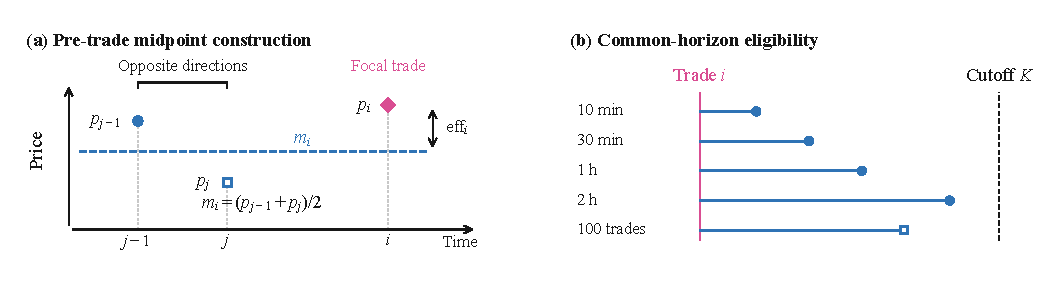
\includegraphics[width=\textwidth]{measurement_timeline}
\Description{Panel a shows the midpoint of an opposite-direction pair completed before the focal buy, and the execution cost relative to that midpoint. Panel b shows five horizon endpoints before the admissibility cutoff.}
\caption{Measurement and horizon eligibility. (a) A completed opposite-direction pair defines the pre-trade midpoint; the focal buy illustrates execution cost. Prices are schematic. (b) The common sample observes all four clock horizons and H100 by cutoff $K$. Endpoint positions illustrate one admissible ordering. Cutoffs R, S, S1 and C are defined in the text.}
\label{fig:timeline}
\end{figure*}

\section{Setting, Data and Measurement}
\label{sec:data}
\paragraph{Contracts and trades.}
A binary contract pays \$1 when its reference outcome occurs and zero otherwise. We map fills in complementary tokens to a common reference outcome; $D=+1$ denotes buying that outcome. The Polymarket v1 archive~\cite{qin2026polymarket} covers November 2022 to April 2026, with 601,934,424 fills in 688,131 markets. Of these markets, 546,187 have a resolved binary payout consistent with the on-chain winner. Fills sharing a market, block timestamp, taker and direction form one trade. Its notional is $u=\sum_j u_j$ and its price is the USD-weighted fill price $p=\sum_j u_jp_j/\sum_j u_j$. Actual outcome-token quantities supply share weights.

\begin{table}[t]
\centering
\caption{Analysis samples. Main: 1--24 h before on-chain resolution, $p\in(0.2,0.8)$, defined midpoint and at least 100 lifetime trades. H100 additionally observes 100 subsequent trades. Clock samples apply the cutoff-specific common-horizon rule.}
\label{tab:flow}
\tabstyle
\begin{tabular}{llrr}
\toprule
Topic & Sample & Markets & Trades \\
\midrule
Yes/No & Main & 11,300 & 2,103,188 \\
 & H100 & 7,819 & 1,774,379 \\
Politics & Main & 4,109 & 516,131 \\
 & H100 & 2,701 & 387,849 \\
Crypto & Main & 2,800 & 1,013,217 \\
 & H100 & 2,360 & 970,065 \\
\midrule
Politics & Clock S & 768 & 179,272 \\
Crypto & Clock S & 2,218 & 795,355 \\
\bottomrule
\end{tabular}

\end{table}

\paragraph{Samples.}
The main Yes/No sample has 2.1 million trades in 11,300 markets (Table~\ref{tab:flow}). The observed 100-trade sample contains 1.8 million trades in 7,819 markets. We also compare sports moneyline and over/under contracts. These samples describe final-day trading at interior prices. Market-level prediction uses an earlier window ending 24 hours before resolution and its own eligibility rules (Section~\ref{sec:prediction}).

\paragraph{Midpoints.}
For consecutive opposite-direction trades, their mean price estimates the midpoint. The prevailing midpoint $m$ is the latest pair completed strictly before the focal trade; the later midpoint $m_{+h}$ uses the latest pair completed by horizon $h$. Pair duration, age and crossing characterize measurement quality. In the main sample, 20.4\% of trades have negative proxy execution cost and 11.9\% of defining pairs are crossed. We examine these features through quote comparisons and alternative pair constructions (Appendix~\ref{app:measurement}).

\paragraph{Observed quotes.}
The pmxt archive records exchange-emitted best bid and ask quotes. We align the reference-axis book to block timestamps using a \QLead-second lead, selected by execution at the touched side (\QMatchPct\%; Figure~\ref{fig:quotes}). The validation keeps a two-sided, uncrossed quote at most 15 minutes old, on every third archive day from 22 February 2026 (\QDays{} days), with each quote-based horizon ending that day. It covers \QTrades{} trades in \QMktsAll{} Politics and Crypto markets. Paired proxy--quote residual differences in the reported cells are at most \QResidMaxAbs{} bp. A second archive, Dome, supplies an additional paired check over October 2025--March 2026 (Appendix~\ref{app:external}). These paired checks address the quote-versus-trade distinction emphasized by Akey et al.~\cite{akey2026quotes}.

\begin{figure}[tbp]
\centering
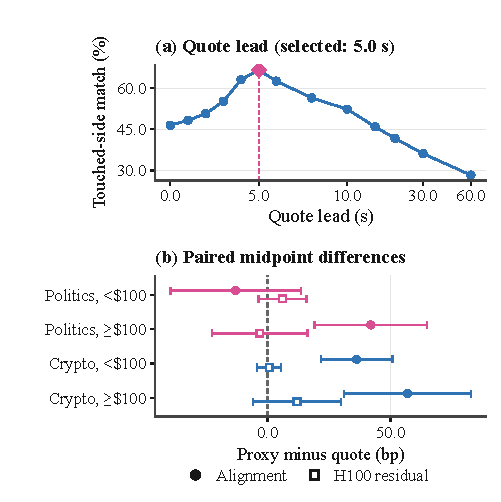
\includegraphics[width=\columnwidth]{quote_validation}
\Description{Two panels show quote-to-trade alignment by lead and paired proxy-minus-quote differences for outcome alignment and the 100-trade residual, with event-cluster intervals.}
\caption{Quote checks separate alignment error from horizon residual error. Lead is chosen by touched-side execution; paired differences use identical trades. Bars are 95.0\% event-cluster intervals.}
\label{fig:quotes}
\end{figure}

\paragraph{Clocks and cutoffs.}
On-chain resolution can lag the event: \PolAfterClose\% of main-window Politics trades occur after the scheduled close, compared with \CryAfterClose\% in Crypto. We use four cutoffs $K$: R, on-chain resolution; S, the earlier of scheduled close and R; S1, S minus one hour; and C, the earlier of S and the last trade pricing the eventual winner below 95.0\% of par. C is a retrospective convergence screen based on the realized winner. Each cutoff's common sample requires the trade's 10-minute, 30-minute, one-hour, two-hour and 100-trade horizons to end by $K$ (Figure~\ref{fig:timeline}). Horizons within a cutoff share observations; cutoffs select different observations. Kalshi calibration research also finds event-time anchoring consequential~\cite{kagan2026calibration}.

\paragraph{Inference and units.}
Standard errors cluster by topic and on-chain resolution date; market clustering and two-way event--calendar-week clustering provide additional inference~\cite{cameron2011robust}. The primary family contains \HeadlineCount{} tests with Benjamini--Hochberg correction. Equivalence tests use fixed margins of 50.0 and 25.0 probability bp. One probability unit equals 10,000.0 bp; 100.0 bp equals one percentage point. USD-weighted margins retain these probability-price units. All forecast gains use baseline minus augmented-model Brier loss, scaled by $10^4$, so positive values favor the augmented model.

\section{Outcome-Based Decomposition}
\label{sec:framework}
Let $Y\in\{0,1\}$ denote the payoff, $p$ the execution price and $D\in\{+1,-1\}$ the trade direction. The prevailing and horizon midpoints are $m$ and $m_{+h}$. Signing in the trade's direction yields
\begin{align}
\underbrace{D(p-m)}_{\eff} &= \underbrace{D(Y-m)}_{\info}+\underbrace{D(p-Y)}_{\RS},\label{eq:i1}\\
\underbrace{D(m_{+h}-m)}_{\PI_h} &= \info+\underbrace{D(m_{+h}-Y)}_{\ovr_h}.\label{eq:i2}
\end{align}
Execution cost $\eff$ combines outcome alignment $\info$ and the gross settlement margin $\RS$ retained by the liquidity-supplying side. Account profit additionally depends on quantities, fees and other positions. A positive mean $\ovr_h$ indicates that the later midpoint lies too far in the trade's direction relative to the payoff.

\paragraph{Conditional pricing benchmark.}
Write $m^*_{i+h}=\mathbb E[Y\mid\mathcal F_{i+h}]$ for the posterior-mean price. With the focal trade in the information set, iterated expectations imply
\begin{equation}
\mathbb E[D_i(m^*_{i+h}-Y)\mid D_i,u_i]=0.\label{eq:orthogonality}
\end{equation}
The focal direction and size are part of the observed history, so the zero-mean forecast error remains orthogonal to direction within each size class. The empirical residual tests this conditional moment. Its interpretation depends on the horizon, eligible observations and information available at the endpoint. Event cutoffs define the corresponding admissible samples.

\paragraph{Within and between markets.}
The payoff is constant within market $g$, giving
\begin{equation}
\mathbb E_g[D(Y-m)] = \underbrace{\bar D_g(Y_g-\bar m_g)}_{\text{between}}+\underbrace{[-\operatorname{Cov}_g(D,m)]}_{\text{within}}.\label{eq:wb}
\end{equation}
The between term relates mean direction to the market's payoff--midpoint gap. The within term measures direction--price timing and is invariant to replacing $Y$. Reversion, midpoint staleness and trading dynamics can all contribute to this covariance. This decomposition identifies the part of measured alignment that explicitly depends on the realized outcome.

\paragraph{Weights and size gradients.}
For any positive weight $w$, the change from an unweighted mean is $\operatorname{Cov}(w,x)/\mathbb E[w]$. Therefore,
\begin{equation}
\mathbb E_w[\RS]-\mathbb E[\RS]
=\frac{\operatorname{Cov}(w,\eff)-\operatorname{Cov}(w,\info)}{\mathbb E[w]}.\label{eq:margin_cov}
\end{equation}
Share- or dollar-weighted margins fall when size covaries more with alignment than with execution cost. Likewise, writing $\Delta$ for large-minus-small differences gives $\Delta\ovr_h=\Delta\PI_h-\Delta\info$: residuals fall with size when alignment rises faster than the response. Across markets, the same weighting identity relates trade-weighted means to market activity.

\section{Order Size and Liquidity Margins}
\label{sec:info}
\subsection{Margins under alternative weights}
\label{sec:rent}
\textbf{The typical trade leaves a positive settlement margin; capital weights shift the average below zero.} On the common observed-horizon sample, the pooled margin is $+\FPRSTr$ bp per trade, compared with \FPRSSh{} bp per actual share and \FPRSUsd{} bp per dollar (Table~\ref{tab:main}; Figure~\ref{fig:weights}(a)). The sign reversal answers RQ1: frequent small interactions and the allocation of traded capital describe different sides of liquidity provision. A positive margin on the typical interaction can coexist with losses concentrated in the orders that carry more capital.

Equation~\eqref{eq:margin_cov} explains the reversal. Capital weighting increases both execution cost and outcome alignment, but the increase in alignment is larger. Execution compensation is outweighed by payoff exposure. Equal-market margins are higher because busy markets have lower margins (Appendix Table~\ref{tab:weight_shifts}). This separation accords with evidence that forecasting and execution are distinct sources of prediction-market returns~\cite{dellavedova2026profits,akey2026who}.

\begin{figure*}[t]
\centering
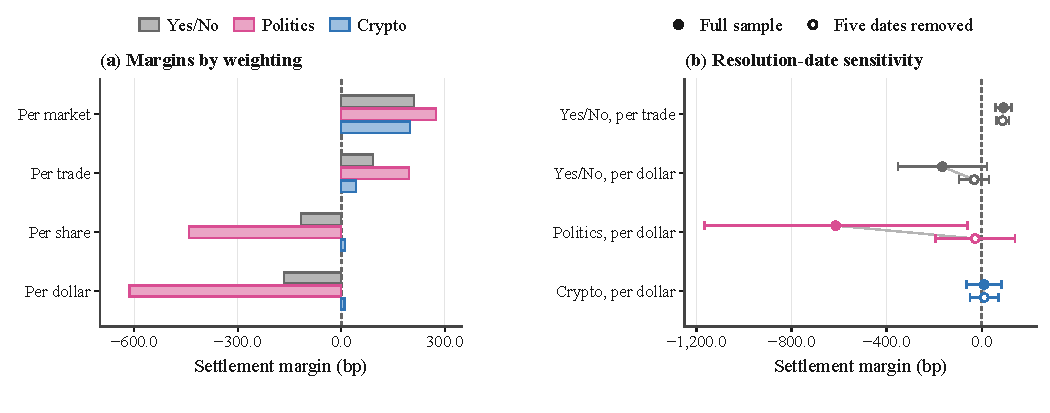
\includegraphics[width=\textwidth]{weights}
\Description{Panel a uses grouped horizontal bars to compare settlement margins under market, trade, actual-share and dollar weights. Panel b pairs full-sample and five-date-deletion estimates with event-cluster intervals.}
\caption{Liquidity margins depend on weighting and resolution-date concentration. (a) Weighted point estimates on the common H100 sample. (b) Full-sample estimates and estimates after dropping the five topic-date clusters with the largest absolute contributions; bars are 95.0\% event-cluster intervals. Actual fill quantities define share weights. Probability bp.}
\label{fig:weights}
\end{figure*}

\begin{table*}[t]
\centering
\caption{Execution costs, alignment, margins, responses and residuals on the observed H100 sample. All five quantities share observations and weights within a row. Parentheses are event-cluster SEs; actual fill quantities define share weights. Probability bp; identities close before rounding.}
\label{tab:main}
\begin{tabular}{llrrrrr}
\toprule
Cell & Weight & $\eff$ & $\info$ & $\RS$ & $\PI_{100}$ & $\ovr_{100}$ \\
\midrule
Yes/No & per trade & 148.9 (3.6) & 57.3 (15.7) & 91.6 (16.6) & 92.2 (4.0) & 34.9 (14.9) \\
Politics & per trade & 235.2 (15.9) & 38.0 (49.7) & 197.2 (57.2) & 137.4 (12.1) & 99.4 (49.0) \\
Crypto & per trade & 114.1 (2.9) & 72.0 (16.0) & 42.1 (16.4) & 84.7 (3.8) & 12.7 (15.3) \\
Sports moneyline & per trade & 81.5 (0.4) & 29.0 (8.0) & 52.6 (8.0) & 42.8 (1.1) & 13.9 (7.9) \\
Over/Under & per trade & 86.9 (1.1) & 22.1 (17.6) & 64.9 (17.7) & 32.9 (3.7) & 10.8 (17.2) \\
\midrule
Yes/No & per market & 296.9 & 86.4 & 210.5 & 142.7 & 56.3 \\
Yes/No & per share & 212.2 & 328.6 & $-$116.4 & 223.2 & $-$105.4 \\
Yes/No & per dollar & 203.8 & 369.0 & $-$165.3 & 231.3 & $-$137.7 \\
\bottomrule
\end{tabular}

\end{table*}

\paragraph{Date concentration.}
The per-trade margin remains positive after removing the five topic-date clusters with the largest absolute contributions. The dollar-weighted mean moves substantially toward zero, from \ConUsd{} to \ConDrop{} bp; its full-sample event-cluster interval already spans zero (Figure~\ref{fig:weights}(b)). Politics shows the strongest concentration: its five largest clusters account for \ConPolTop\% of absolute contributions. Date concentration preserves the positive per-interaction result while qualifying the capital-weighted average.

Shared outcomes reduce the independent information in transaction counts. Weight-sensitive Polymarket returns in Cardozo and Rivero-Wildemauwe~\cite{cardozo2026favorite} similarly motivate reporting aggregation units and concentration.

\paragraph{Fill quantities and prices.}
Share weights use observed outcome-token quantities summed over fills. Replacing the USD-weighted execution price with its share-weighted counterpart changes the pooled per-trade margin by only \FPRSDiff{} bp and preserves the negative actual-share margin. Appendix Table~\ref{tab:fill} also reports the constructed quantity $u/p$. Its difference from observed shares follows from complementary tokens executing at their native prices, including $1-p$ on the reference axis. Thus, the reversal survives a fill-level price check.

\subsection{Outcome-related and timing components}
\textbf{Politics and Crypto have different sources of the size gradient.} Pooled alignment in the main sample is predominantly within-market direction--price covariance (Table~\ref{tab:wb_size}). Pooling, however, conceals a consequential topic difference. In Politics, alignment rises strongly with order size, and most of the increase lies in the between component. Large political orders more often point toward outcomes that eventually pay relative to the market's mean midpoint. Small political orders have a negative between component, offset by positive within-market timing. Their near-zero total alignment therefore combines two economically different relationships.

In Crypto, the size gradient lies mainly in the within component. Larger orders tend to trade at more favorable points along the midpoint path, while the between component provides much less of the increase. Since the within term is unchanged when the market's outcome is replaced, it can arise from price timing, reversion or proxy staleness. Thus, the political gradient involves outcomes, while Crypto primarily reflects timing.

\begin{table}[t]
\centering
\caption{The Politics size gradient lies mainly between markets; the Crypto gradient lies mainly within markets. Main final-day sample, eq.~\eqref{eq:wb}. Probability bp; event-cluster SEs.}
\label{tab:wb_size}
\begin{tabular}{llrrr}
\toprule
Topic & Size & $\info$ & Between & Within \\
\midrule
Politics & $<\$100$ & \ensuremath{-}0.5 (33.9) & \ensuremath{-}126.6 (36.4) & 126.1 (10.3) \\
Politics & \$100--1k & 384.1 (90.4) & 169.7 (94.6) & 214.5 (12.2) \\
Politics & $\ge\$1$k & 885.3 (203.2) & 713.0 (197.0) & 172.3 (16.7) \\
Politics & all & 68.2 (38.5) & \ensuremath{-}75.1 (43.1) & 143.3 (9.7) \\
\addlinespace
Crypto & $<\$100$ & 67.1 (17.5) & 35.3 (17.2) & 31.8 (3.9) \\
Crypto & \$100--1k & 143.2 (23.8) & \ensuremath{-}23.4 (22.2) & 166.6 (7.9) \\
Crypto & $\ge\$1$k & 218.7 (43.7) & \ensuremath{-}22.8 (41.9) & 241.4 (14.5) \\
Crypto & all & 82.2 (15.7) & 24.1 (15.2) & 58.2 (3.8) \\
\addlinespace
Yes/No & all & 76.0 (13.9) & 0.9 (14.3) & 75.1 (3.4) \\
\bottomrule
\end{tabular}

\end{table}

Figure~\ref{fig:size} connects the alignment gradient to margins and residuals on the observed H100 sample. Large Politics orders have higher alignment and lower margins than small orders. Their price response also increases, but less than alignment; the resulting large-minus-small residual contrast is \ThTwo{} bp. This links liquidity margins in RQ1 to conditional pricing in RQ2.

\begin{figure*}[t]
\centering
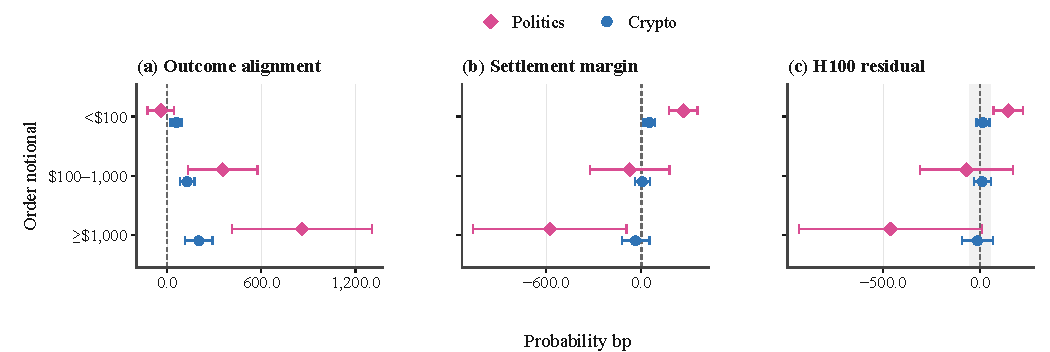
\includegraphics[width=\textwidth]{size_pricing}
\Description{Three horizontal interval plots compare alignment, settlement margin and the H100 residual across order-size bins. Politics uses pink diamonds and Crypto blue circles, with 95 percent event-cluster intervals.}
\caption{Order size separates alignment, liquidity margins and subsequent pricing. Estimates use the observed H100 sample; bars are 95.0\% event-cluster intervals. Politics: pink diamonds; Crypto: blue circles. The shaded residual band marks $\pm50.0$ bp as a visual equivalence benchmark. Probability bp.}
\label{fig:size}
\end{figure*}

\section{Conditional Pricing after Small Political Orders}
\label{sec:over}
\subsection{Trade-count horizons and direct contrasts}
\textbf{Small Politics orders leave a positive residual with a size gradient.} After 100 subsequent trades, their residual is \PolSmall{} bp and survives correction across the primary test family. The direct large-minus-small contrast is \ThTwo{} bp, with an interval excluding zero under both event and two-way clustering (Table~\ref{tab:contrasts}). The regression accounts for the shared covariance between size classes. This comparison establishes a size gradient even though the large-order level itself is imprecisely estimated.

A positive residual means that the later midpoint averages above the payoff after a buy and below it after a sell. This conditional moment describes the order group; individual trades can still precede informative updates.

\begin{table}[t]
\centering
\caption{Direct residual contrasts share the covariance from one regression on the observed H100 sample. Parentheses are topic-by-resolution-date SEs; the final column adds calendar-week clustering. Probability bp.}
\label{tab:contrasts}
\begin{tabular}{lrr}
\toprule
Contrast & Estimate & Two-way SE \\
\midrule
Politics, below \$100 & 144.4 (38.8) & 37.2 \\
Politics, large minus small & \ensuremath{-}606.9 (229.5) & 209.8 \\
Politics minus Crypto, small & 130.7 (42.4) & 37.7 \\
\addlinespace
Alignment, large minus small & 898.5 (221.2) & 197.7 \\
Response, large minus small & 291.6 (42.1) & 44.8 \\
\bottomrule
\end{tabular}

\end{table}

Small Politics orders also exceed small Crypto orders in the direct topic comparison. Crypto's small-order residual is close to zero and passes the fixed $\pm50.0$ bp equivalence test; the tighter $\pm25.0$ bp test remains inconclusive. The wider band also contains pooled Crypto, its medium orders, sports moneyline and Over/Under under the corresponding tests. Equivalence concerns the precision of a bounded average residual. The imprecise Crypto large-order estimate supports a weaker conclusion, since a point estimate near zero alone cannot establish a small effect.

\subsection{Clock horizons and event eligibility}
\textbf{The small-Politics residual persists over fixed amounts of real time.} Figure~\ref{fig:clock} shows a positive political pattern from ten minutes through two hours. At one hour it is \PolSHourR{} bp under on-chain resolution and remains positive under the earlier cutoffs. Small Crypto estimates stay near zero, and the Politics--Crypto difference is positive throughout the cutoff--horizon grid (Appendix Table~\ref{tab:clock}). The clock design addresses a limitation of trade-count horizons: the same number of later trades can represent very different opportunities for updating across markets.

\begin{figure*}[t]
\centering
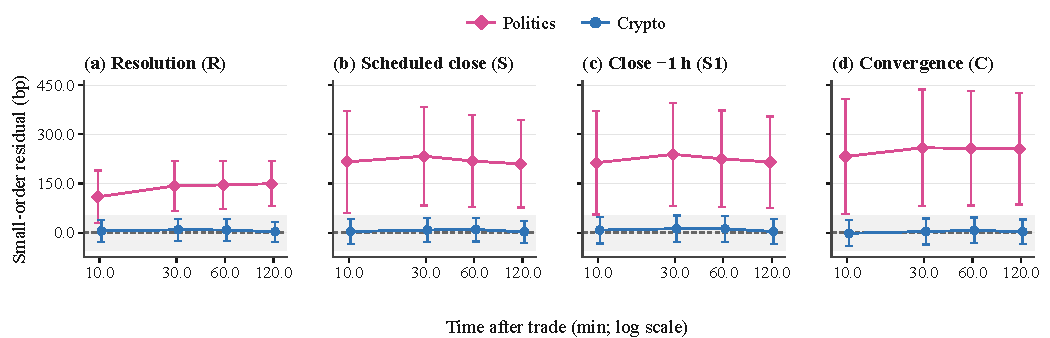
\includegraphics[width=\textwidth]{clock_profile}
\Description{Four cutoff panels show small-order pricing residuals at ten minutes, thirty minutes, one hour and two hours. Politics estimates are positive; Crypto estimates cluster near zero. Each panel uses its own common sample.}
\caption{Small political orders retain a directional residual across real-time horizons. Each panel uses the common sample of its cutoff; bars are 95.0\% event-cluster intervals. The shaded band marks $\pm50.0$ bp. Time is in elapsed minutes on a log scale. Each cutoff has its own eligible observations. Probability bp.}
\label{fig:clock}
\end{figure*}

Each panel holds trades fixed across horizons. S and C select fewer markets, so their larger political estimates can reflect composition as well as timing. The positive sign persists before scheduled close and retrospective convergence. Matching on midpoint decile, time to resolution and quarter, with log market trade count, preserves the topic difference (Appendix Table~\ref{tab:clock}).

\paragraph{Retention and direction.}
The H100 rule retains \RetPol\% of Politics small orders and \RetCry\% of Crypto small orders. Its median elapsed horizon is longer in Politics, reinforcing the value of clock comparisons. Small- and large-order settlement margins retain their signs among kept and dropped trades, while medium-order signs differ (Table~\ref{tab:retention}). Selection is therefore relevant to the composition of the sample, and the unobserved H100 residuals of dropped trades remain unresolved. Direction is a separate source of sensitivity. Using the tick rule preserves a positive Politics small-order residual while materially reducing its magnitude; rebuilding the midpoint from tick-rule switches yields a similar change (Table~\ref{tab:direction}). The direction checks support the qualitative sign with a narrower claim about the stability of its numerical level.

\begin{table}[tbp]
\centering
\caption{H100 retention, elapsed time and settlement margins for retained and dropped trades. Probability bp; event-cluster SEs.}
\label{tab:retention}
\tabstyle
\begin{tabular}{lrrrrr}
\toprule
Cell & Kept & Median & $p_{90}$ & RS kept & RS dropped \\
\midrule
Politics $<\$100$ & 73.9\% & 2.2 h & 10.9 h & 265.3 (45.3) & 358.7 (29.7) \\
Politics \$100--1k & 80.7\% & 1.2 h & 8.7 h & \ensuremath{-}72.2 (128.0) & 98.6 (71.0) \\
Politics $\ge\$1$k & 90.3\% & 0.7 h & 5.6 h & \ensuremath{-}575.2 (246.5) & \ensuremath{-}494.9 (199.6) \\
Crypto $<\$100$ & 95.9\% & 0.7 h & 4.2 h & 50.7 (18.2) & 17.5 (48.4) \\
Crypto \$100--1k & 95.3\% & 0.6 h & 4.1 h & 7.1 (24.0) & \ensuremath{-}140.1 (86.6) \\
Crypto $\ge\$1$k & 93.2\% & 0.5 h & 4.2 h & \ensuremath{-}36.1 (44.3) & \ensuremath{-}181.6 (154.1) \\
\bottomrule
\end{tabular}

\end{table}

\begin{table}[tbp]
\centering
\caption{Direction sensitivity on the same H100 trades and fixed midpoint. Tick rule carries the last nonzero price change; zero changes cover \DirZero\% of trades. Difference: tick minus on-chain. Probability bp.}
\label{tab:direction}
\tabstyle
\begin{tabular}{lrrrr}
\toprule
Cell & Agree & On-chain $\ovr_{100}$ & Tick rule & Difference \\
\midrule
Yes/No & 75.2\% & 34.9 & 4.6 & \ensuremath{-}30.3 (11.5) \\
Politics $<\$100$ & 76.9\% & 144.4 & 64.8 & \ensuremath{-}79.6 (34.2) \\
Politics $\ge\$1$k & 90.4\% & \ensuremath{-}462.5 & \ensuremath{-}395.7 & 66.8 (27.9) \\
Crypto $<\$100$ & 72.4\% & 13.8 & 4.6 & \ensuremath{-}9.1 (14.9) \\
\bottomrule
\end{tabular}

\end{table}

\paragraph{Quotes and periods.}
Dome quotes change the Politics small-order residual little on identical trades, although archive coverage limits extrapolation. Across four resolution periods, one-hour point estimates stay positive under R, S and C with period-specific uncertainty (Appendix Table~\ref{tab:forward}). Forward scoring tests whether this recurrence supports forecast improvement.

Figure~\ref{fig:proxy} compares small-order residuals across alternative midpoint constructions. These main-sample diagnostics cap unavailable H100 endpoints, so their levels differ from the observed-horizon estimates. The political sign persists across constructions, while the choice of midpoint changes its magnitude.

\begin{figure}[tbp]
\centering
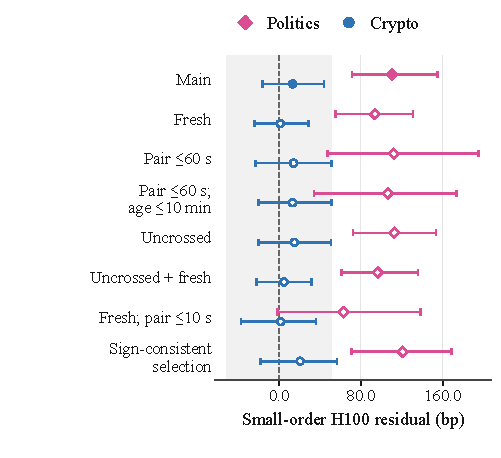
\includegraphics[width=\columnwidth]{proxy_sensitivity}
\Description{A forest plot compares capped-endpoint small-order residuals across eight midpoint constructions in Politics and Crypto.}
\caption{Small-order residuals across midpoint constructions on the main sample, with capped H100 endpoints. Filled markers show the main construction; open markers show alternative pair constructions and the sign-consistent selection. Bars are 95.0\% market-cluster bootstrap intervals. Shading: $\pm50.0$ bp.}
\label{fig:proxy}
\end{figure}

\section{Forecasting and Generalization}
\label{sec:prediction}
\subsection{Forward prediction conditional on the midpoint}
An expanding-window outcome logit uses the one-hour midpoint, a Politics indicator and direction-by-topic-by-size terms. Each test quarter uses coefficients fitted on earlier resolution quarters. On the S common sample, the small-Politics direction coefficient is negative in all six test quarters, matching the positive residual's sign. Forecast gains nonetheless vary across quarters, and the pooled Politics Brier interval spans zero (Figure~\ref{fig:forecast}). C gives a similar pattern (Appendix Table~\ref{tab:fwdpred}).

For RQ3, stable coefficient signs establish a recurring association. Forecast improvement additionally requires learning its magnitude on earlier events and maintaining it later. Paired forward losses test that requirement and allow both gains and deterioration.

\begin{figure}[t]
\centering
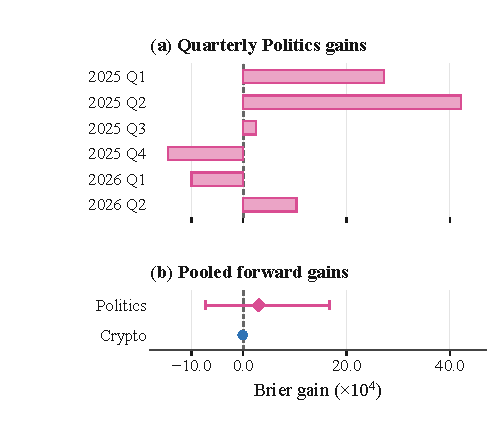
\includegraphics[width=\columnwidth]{forward_prediction}
\Description{Panel a shows quarterly Politics Brier gains as diverging bars. Panel b shows pooled Politics and Crypto gains with paired 95 percent event-cluster intervals. Positive gains favor the flow-augmented model.}
\caption{Forward forecast gains vary across periods. (a) Quarterly Politics gains on the S common sample. (b) Pooled gains with paired 95.0\% event-cluster intervals. Gain is price-only minus flow-model Brier loss, $\times10^4$. Coefficients appear in Table~\ref{tab:fwdpred}.}
\label{fig:forecast}
\end{figure}

\subsection{Market-level flow and price calibration}
For each market $g$, we compute the dollar imbalance within each size class $k$: $b_{k,g}=\sum_{i\in\mathcal T_{k,g}}D_i u_i/\sum_{i\in\mathcal T_{k,g}}u_i$. Here $\mathcal T_{s,g}$ contains orders below \$100 and $\mathcal T_{l,g}$ orders of at least \$1,000 over the history ending 24 hours before resolution. We estimate
\begin{equation}
\operatorname{logit}\Pr(Y_g=1)=\alpha+\gamma\operatorname{logit}(p_g)+\beta_s b_{s,g}+\beta_l b_{l,g}+\eta_{c(g)}.\label{eq:joint_flow}
\end{equation}
Here $p_g$ is the latest switch midpoint by the window endpoint. Eligibility requires at least 200 lifetime trades, 20 window trades, $100p_g\in(2.0,98.0)$ and observed imbalances in both size classes. All nested models share markets and five event-grouped folds. Paired loss intervals use 1,000 event-cluster draws.

Politics has a negative small-flow coefficient conditional on the window-end price, while Crypto's estimate is close to zero (Table~\ref{tab:joint_flow}). More small-order buying therefore accompanies fewer Yes resolutions at a given price in Politics, echoing the trade-level residual in an earlier market window. The Politics joint-flow gain is \EdJointPolGain{} $\times10^{-4}$ on 1,559 markets, with an interval spanning zero. Dollar imbalance aggregates a market history, while the residual follows an individual order; their signs agree across distinct eligible populations.

\begin{table}[tbp]
\centering
\caption{Joint-flow logits on common markets ending 24 h before resolution. Coefficients and their event-cluster SEs are multiplied by 10. Brier gains are $\times10^4$, with paired event-cluster intervals.}
\label{tab:joint_flow}
\tabstyle
\begin{tabular}{lrrrr}
\toprule
Segment & $n$ & \thead{Small-flow\\$10\beta$ (SE)} & \thead{Large-flow\\$10\beta$ (SE)} & \thead{$10^4\Delta$Brier\\{[95.0\% CI]}} \\
\midrule
Yes/No & 5,755 & -6.6 (2.1) & +1.3 (0.7) & +4.6 [-1.6, +10.8] \\
Politics & 1,559 & -13.3 (4.0) & +2.2 (1.3) & +18.7 [-5.6, +41.5] \\
Crypto & 2,825 & -0.3 (3.0) & +0.6 (1.2) & -4.3 [-8.0, -0.6] \\
Moneyline & 5,376 & -0.4 (0.9) & -0.1 (0.4) & -1.4 [-2.8, +0.0] \\
\bottomrule
\end{tabular}

\end{table}

\begin{figure*}[t]
\centering
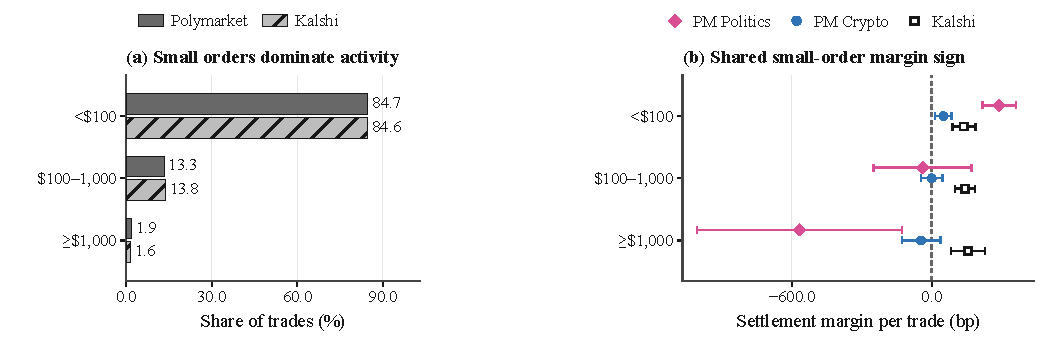
\includegraphics[width=\textwidth]{cross_platform}
\Description{Panel a compares cash-bin trade shares in Polymarket and Kalshi. Small trades dominate both. Panel b shows positive small-order settlement margins in Polymarket Politics, Polymarket Crypto and Kalshi, with different size gradients.}
\caption{Cross-venue regularities and differences. (a) Trade shares by cash bin. (b) Gross settlement margins per trade; bars are 95.0\% intervals using each source's event clusters. Polymarket uses the main Yes/No sample 1--24 h before on-chain resolution; Kalshi uses 1--24 h before exchange close. Different events and clocks preclude a causal venue comparison. Kalshi squares are hollow; Polymarket topics retain their colors and markers.}
\label{fig:crossplatform}
\end{figure*}

A separate comparison uses 5,799 markets and a price spline with knots fixed before scoring. Allowing a flexible price relationship helps assess whether flow merely proxies for a misspecified calibration curve. Small-flow gains relative to the linear-logit price baseline remain uncertain in both grouped cross-validation and forward evaluation (Table~\ref{tab:spline}). The spline alone also underperforms the linear baseline in the forward sample. Additional flexibility can therefore absorb in-sample variation without improving later predictions. Across the evaluated designs, RQ3 yields a recurring direction coefficient alongside imprecise incremental gains; the evidence supports conditioning the interpretation of a forecast on participation, with predictive deployment requiring further validation.

\subsection{Cross-platform regularities and scope}
\label{sec:kalshi}
\textbf{Small orders dominate activity and leave positive settlement margins in both venues.} Kalshi contributes \KalTrades{} trades in \KalMkts{} settled binary markets, observed 1--24 h before exchange close with the same interior-price and cash-bin thresholds. Figure~\ref{fig:crossplatform}(a) compares these trades with Polymarket's main Yes/No sample: orders below \$100 account for over four-fifths of transactions in each venue. Their margins are positive in Kalshi and in both focal Polymarket topics (panel b). This common pattern links broad participation to compensation on the typical small interaction. It accords with Kalshi maker--taker evidence~\cite{burgi2026makers,becker2026microstructure} and Polymarket liquidity-provider results~\cite{akey2026who}; our gross per-trade margins and those papers' returns or account profits retain different weights and targets.

\paragraph{Size gradients and weighting.}
Kalshi margins remain positive under both trade and dollar weights within every cash bin (Appendix Table~\ref{tab:extkalshi}). Its absolute large-minus-small contrast is imprecise, while within-market cash ranks produce a positive high-minus-low contrast of \KalRank{} bp. Hence, positive small-order compensation generalizes more readily than a particular slope in absolute dollars. Relative ranks measure scale against local activity; dollar bins measure committed cash, and the two need not encode the same participant composition. Le~\cite{le2026decomposing} likewise finds cross-platform political calibration patterns alongside a size gradient that is not robust across venues. That result concerns calibration slopes; ours concerns direction-signed settlement margins.

\paragraph{Prediction and comparability.}
Kalshi small-flow augmentation worsens forward Brier loss, whereas joint small/large flow improves it by \KalBothG{} $\times10^{-4}$ in a separate, smaller cohort (Appendix Table~\ref{tab:extkalshipred}). The positive joint result shows that order flow can add information in an eligible population; the two cohorts provide separate comparisons with their own price baselines. Together with Polymarket's uncertain gains, these results make forecast improvement conditional on both features and the evaluated population.

This comparison uses different events and clocks. Kalshi's fetch-time books supply no pre-trade midpoint history, so $D(p-Y)$ tests margins. Contract design and settlement semantics constrain comparison~\cite{lee2026derivatives,gebele2026semantic}. Matched studies find context-dependent leadership and pricing gaps~\cite{ng2026discovery,aktug2026discovery,rothschild2014misalignment,zitzewitz2026limits}. Shared participation and small-order compensation therefore coexist with sample-specific size gradients.

\section{Related Work}
\paragraph{Collective forecasts and participation.}
Laboratory and political markets aggregate dispersed information~\cite{plott1988rational,forsythe1992anatomy,wolfers2004prediction,arrow2008promise}; related-event and field designs extend this evidence~\cite{hanson2003combinatorial,berg2008accuracy,berg2008results,cowgill2015corporate}. Web platforms expose contribution quality and investor behavior~\cite{horvat2023hidden,soska2021derivatives,kawai2023neighbor,victor2021wash}. We distinguish frequent interactions from capital exposure using a common binary-payoff benchmark.

\paragraph{Execution and price formation.}
Microstructure models connect order flow, adverse selection and price discovery~\cite{kyle1985continuous,glosten1985bid,easley1987price,glosten1988estimating,hasbrouck1991measuring,huang1997components,madhavan1997why}. Prediction-market work studies liquidity and strategies~\cite{tetlock2008liquidity,rothschild2016trading,bossaerts2024price}, execution versus forecasting~\cite{dellavedova2026profits}, maker--taker outcomes~\cite{burgi2026makers,becker2026microstructure,akey2026who} and quote updates~\cite{akey2026quotes}. Our within/between decomposition and quote checks connect settlement margins to subsequent direction-signed errors, without identifying order size as an exogenous treatment.

\paragraph{Conditional calibration and venue comparisons.}
Heterogeneous beliefs complicate price interpretation~\cite{manski2006interpreting,wolfers2006interpreting}; calibration varies with price, horizon and aggregation~\cite{snowberg2010explaining,page2013prediction,cardozo2026favorite,reichenbach2026exploring,kagan2026calibration}. Contemporary studies examine order books~\cite{dubach2026anatomy} and political activity~\cite{tsang2026anatomy,tsang2026political,chen2025political}. Le~\cite{le2026decomposing} documents political calibration commonalities alongside unstable cross-venue size effects. Matched studies find conditional leadership and persistent pricing differences~\cite{ng2026discovery,aktug2026discovery,rothschild2014misalignment,zitzewitz2026limits}; design and settlement affect matching~\cite{lee2026derivatives,gebele2026semantic}. We examine an order-conditioned price moment and separately assess forward gains, using Kalshi to distinguish shared small-order margins from sample-specific size gradients.

\newpage
\section{Discussion and Conclusion}
\label{sec:discuss}
\paragraph{Participation and liquidity.}
Positive per-trade margins coexist with negative capital-weighted point estimates and concentrated outcome exposure. Politics' size gradient involves payoffs; Crypto's mainly reflects price timing. Kalshi shares small-order dominance and positive small-order margins, with different size gradients. Thus, broad participation and compensation on small interactions generalize more readily than an absolute-dollar ranking of informedness.

\paragraph{Conditional forecasts.}
Small political orders leave positive residuals across horizons, event screens and resolution periods, alongside uncertain forward gains. Kalshi's joint-flow gain in its eligible cohort reinforces the distinction between a conditional error and a usable forecast correction. Prospective evaluation should fix features, bins and cutoffs, then report paired event losses.

\paragraph{Mechanisms and scope.}
Quote updating, partisan demand and reference-price access offer possible explanations; text classes and BTC features provide descriptive checks. Identifying mechanisms requires contemporaneous references, inventories and repeated participation. Quote coverage is selective; event screens use metadata and retrospective convergence. Gross settlement margins exclude fees and inventory, and midpoint residuals omit executable spreads and depth. These boundaries preserve the distinction between conditional association, trading profit and causal platform effects.

\label{paper:body_end}
\clearpage
\nobalance
\phantomsection\label{paper:references_start}
\bibliographystyle{ACM-Reference-Format}
\bibliography{ref}
\appendix
\renewcommand{\floatpagefraction}{0.95}
\renewcommand{\dblfloatpagefraction}{0.95}
\renewcommand{\topfraction}{0.95}
\renewcommand{\dbltopfraction}{0.95}
\renewcommand{\textfraction}{0.05}
\setcounter{topnumber}{4}
\setcounter{bottomnumber}{4}
\setcounter{totalnumber}{8}
\setcounter{dbltopnumber}{4}
\renewcommand{\thetable}{S\arabic{table}}
\renewcommand{\thefigure}{S\arabic{figure}}
\renewcommand{\theHtable}{S\arabic{table}}
\renewcommand{\theHfigure}{S\arabic{figure}}
\setcounter{table}{0}
\setcounter{figure}{0}
\phantomsection\label{paper:appendix_start}

\section{Sample Construction, Fills and Concentration}
\label{app:defs}
On-chain payout events define resolution; block timestamps are interpolated at 2.1 seconds per block. The 100-trade sample retains 75.1\% of main Politics trades and 95.7\% of Crypto trades. Overall median horizons are 2.0 hours in Politics and 42.7 minutes in Crypto (90th percentiles 10.5 and 4.2 hours). Median on-chain delays after scheduled close are 14.6 and 2.4 hours. Common-sample trade counts under R, S and C are \PolNR, \PolNS{} and \PolNC{} in Politics and \CryNR, \CryNS{} and \CryNC{} in Crypto. Ordering simultaneous trades by taker address changes alignment by \OrdDiff{} bp (SE \OrdSE).

\begin{table}[!htbp]
\centering
\caption{Fill prices and actual share weights on the common H100 sample. The final column uses a share-weighted execution price. Probability bp.}
\label{tab:fill}
\begin{tabular}{lrrrr}
\toprule
Weight & $\eff$ & $\info$ & $\RS$ & $\RS$, share price \\
\midrule
per trade & 148.9 & 57.3 & 91.6 & 92.1 \\
per share, observed & 212.2 & 328.6 & \ensuremath{-}116.4 & \ensuremath{-}112.3 \\
per share, $u/p$ & 198.4 & 441.0 & \ensuremath{-}242.6 & \ensuremath{-}239.8 \\
per dollar & 203.8 & 369.0 & \ensuremath{-}165.3 & \ensuremath{-}162.5 \\
\bottomrule
\end{tabular}

\end{table}
\begin{table}[!htbp]
\centering
\caption{Normalized covariance shifts on the common H100 sample. Market shift: per trade minus per market; order shift: per USD minus per trade. Probability bp.}
\label{tab:weight_shifts}
\begin{tabular}{lrr}
\toprule
Component & Market shift & Order shift \\
\midrule
Execution cost & -148.0 & +54.9 \\
Alignment & -29.1 & +311.7 \\
Settlement margin & -118.9 & -256.9 \\
\bottomrule
\end{tabular}

\end{table}

\subsection{Resolution-date concentration}
\label{app:concentration}
Table~\ref{tab:concentration} ranks clusters by absolute contribution within topic and weight. Deletion diagnoses influence on a changing population. Table~\ref{tab:concentration_dates} gives Politics' largest dollar-weighted contributors and their volume shares.
\begin{table}[!htbp]
\centering
\caption{Settlement margins and deletion of influential topic-date clusters. Probability bp; parentheses are event-cluster SEs. The final column is the five largest clusters' share of absolute contributions.}
\label{tab:concentration}
\tabstyle
\begin{tabular}{lrrrr}
\toprule
Sample & Full sample & Drop 5 dates & Drop largest & Top 5 share \\
\midrule
Yes/No, per trade & 91.6 (16.6) & 87.7 (13.6) & 100.0 & 6.9\% \\
Yes/No, per dollar & \ensuremath{-}165.3 (95.5) & \ensuremath{-}32.0 (32.0) & \ensuremath{-}75.5 & 23.0\% \\
Politics, per dollar & \ensuremath{-}613.9 (282.2) & \ensuremath{-}27.5 (85.6) & \ensuremath{-}302.3 & 55.1\% \\
Crypto, per dollar & 9.8 (37.2) & 10.8 (30.9) & \ensuremath{-}5.8 & 11.8\% \\
\bottomrule
\end{tabular}

\end{table}
\begin{table}[!htbp]
\centering
\caption{The five largest Politics resolution-date contributors by absolute dollar-weighted contribution. Dollar shares are percentages; contributions are probability bp.}
\label{tab:concentration_dates}
\tabstyle
\begin{tabular}{lrr}
\toprule
Resolution date & Dollar share & Contribution \\
\midrule
2026-02-28 & 43.1\% & \ensuremath{-}363.1 \\
2025-06-22 & 12.7\% & \ensuremath{-}84.1 \\
2025-06-04 & 4.6\% & \ensuremath{-}61.5 \\
2026-04-08 & 16.5\% & \ensuremath{-}56.5 \\
2025-06-13 & 4.6\% & \ensuremath{-}30.0 \\
\bottomrule
\end{tabular}

\end{table}

\section{Quote Validation and Measurement Sensitivity}
\label{app:measurement}
\label{sec:quotes}
\label{sec:proxy}
The pmxt source is \nolinkurl{Joseph3222/polymarket-orderbook} (CC BY 4.0). Script 13a retrieves the needed row groups, covering each trade's preceding 15 minutes and subsequent two hours plus its H100 endpoint. Complementary books are mirrored onto the reference axis. Table~\ref{tab:quotes} and Figure~\ref{fig:quotes} compare identical trades. With $e=m-m^q$, alignment error is $-De$ and the horizon residual error is $De_{+h}$. Median proxy age is 56.0 s pooled, 142.0 s in Politics and 28.0 s in Crypto. Fresh pairs cover 41.2\% of main trades. Capped-endpoint Politics small/large residuals are $+110.2/-418.7$ bp; observed H100 estimates are $+144.4/-462.5$ bp. Figure~\ref{fig:proxy} compares small-order residuals across midpoint constructions. The full topic-by-size grid is supplied with the analysis outputs.
\begin{table*}[!tbp]
\centering
\caption{Quoted midpoint estimates and paired proxy-minus-quote differences on pmxt-covered main-sample trades. Clock residuals apply the R/S common-horizon rules and same-day quote availability. Market/trade counts describe the pre-trade match. Probability bp; event-cluster SEs.}
\label{tab:quotes}
\tabstyle
\begin{tabular}{lrrrrrrrrrr}
\toprule
 & & & \multicolumn{2}{c}{$\info$} & \multicolumn{2}{c}{$\ovr_{1\mathrm h}$, R} & \multicolumn{2}{c}{$\ovr_{1\mathrm h}$, S} & \multicolumn{2}{c}{$\ovr_{100}$} \\
\cmidrule(lr){4-5}\cmidrule(lr){6-7}\cmidrule(lr){8-9}\cmidrule(lr){10-11}
Cell & Markets & Trades & Quote & Proxy$-$quote & Quote & Proxy$-$quote & Quote & Proxy$-$quote & Quote & Proxy$-$quote \\
\midrule
Yes/No & 491 & 69,008 & 114.2 (47.9) & 20.8 (6.9) & 37.7 (52.1) & \ensuremath{-}4.9 (2.9) & 58.7 (66.3) & \ensuremath{-}3.0 (3.4) & 45.8 (48.6) & 2.8 (2.4) \\
Politics & 287 & 28,294 & 221.7 (70.9) & \ensuremath{-}4.4 (12.7) & 36.2 (103.2) & \ensuremath{-}4.7 (4.3) & 86.2 (192.0) & 0.4 (5.4) & 38.2 (86.7) & 4.3 (5.1) \\
\quad $<\$100$ & 284 & 23,846 & 185.7 (116.7) & \ensuremath{-}13.0 (13.5) & 51.6 (132.5) & \ensuremath{-}5.1 (4.7) & 139.3 (249.4) & 1.6 (5.7) & 81.4 (120.0) & 6.1 (5.0) \\
\quad $\ge\$100$ & 188 & 4,448 & 414.8 (243.6) & 42.0 (11.7) & \ensuremath{-}31.5 (85.8) & \ensuremath{-}3.1 (2.9) & \ensuremath{-}141.8 (76.9) & \ensuremath{-}4.6 (6.9) & \ensuremath{-}144.4 (190.0) & \ensuremath{-}3.1 (9.9) \\
Crypto & 204 & 40,714 & 39.5 (61.3) & 38.3 (7.4) & 38.5 (55.7) & \ensuremath{-}5.0 (3.9) & 49.5 (61.7) & \ensuremath{-}4.2 (4.2) & 50.4 (58.0) & 1.8 (2.5) \\
\quad $<\$100$ & 202 & 36,635 & 31.7 (67.0) & 36.2 (7.4) & 44.8 (62.3) & \ensuremath{-}6.5 (4.1) & 53.2 (69.4) & \ensuremath{-}5.9 (4.3) & 45.5 (62.7) & 0.6 (2.5) \\
\quad $\ge\$100$ & 160 & 4,079 & 109.5 (73.8) & 56.9 (13.2) & \ensuremath{-}17.2 (86.1) & 8.5 (6.9) & 13.4 (94.6) & 12.7 (6.7) & 93.4 (76.2) & 12.0 (9.2) \\
\bottomrule
\end{tabular}

\end{table*}

\paragraph{Quote error by measurement state.}
Table~\ref{tab:quote_error} separates signed error, absolute error and negative-cost frequency. Stale/crossed pairs have larger absolute errors; proxy costs are more often negative. Overlapping rows classify the same trades by measurement state.
\begin{table*}[!tbp]
\centering
\caption{Proxy error on pmxt-matched trades. With $e=m-m^q$, $De$ is signed proxy error and $|e|$ is mean absolute error, in probability bp. Outside is the percentage of proxy midpoints outside the quoted spread. The last column reports negative execution-cost percentages for proxy/quote midpoints; parentheses are event-cluster SEs. Rows overlap.}
\label{tab:quote_error}
\tabstyle
\begin{tabular}{lrrrrr}
\toprule
Trades & $n$ & $De$ & $|e|$ & Outside & $D(p-m)<0$ \\
\midrule
All trades & 69,008 & \ensuremath{-}20.8 (6.9) & 242.9 & 42.7\% & 20.7 / 7.4\% \\
\addlinespace
Politics $<\$100$ & 23,846 & 13.0 (13.5) & 279.4 & 31.1\% & 17.0 / 6.4\% \\
Politics $\ge\$100$ & 4,448 & \ensuremath{-}42.0 (11.7) & 186.1 & 29.2\% & 9.6 / 5.5\% \\
Crypto $<\$100$ & 36,635 & \ensuremath{-}36.2 (7.4) & 225.1 & 50.0\% & 24.1 / 7.9\% \\
Crypto $\ge\$100$ & 4,079 & \ensuremath{-}56.9 (13.2) & 252.6 & 59.0\% & 24.7 / 10.9\% \\
\addlinespace
Fresh pair & 29,243 & \ensuremath{-}2.3 (3.7) & 162.9 & 31.5\% & 17.3 / 7.4\% \\
2--5 trades old & 31,134 & \ensuremath{-}16.8 (8.2) & 258.6 & 46.9\% & 23.1 / 7.5\% \\
$>5$ trades old & 8,631 & \ensuremath{-}98.1 (21.9) & 457.7 & 65.1\% & 23.8 / 7.1\% \\
\addlinespace
Crossed pair & 9,033 & 20.7 (13.1) & 302.0 & 64.4\% & 39.4 / 11.7\% \\
Uncrossed pair & 59,975 & \ensuremath{-}27.0 (6.5) & 234.0 & 39.4\% & 17.9 / 6.8\% \\
\addlinespace
Quoted spread $\le$2c & 30,679 & \ensuremath{-}23.7 (5.8) & 147.3 & 54.5\% & 24.7 / 7.2\% \\
Quoted spread $>$2c & 38,329 & \ensuremath{-}18.5 (10.7) & 319.5 & 33.2\% & 17.5 / 7.6\% \\
\bottomrule
\end{tabular}

\end{table*}

\subsection{Within/between checks and simulation}
\label{app:wb}
Politics alignment is $68.2=-75.1+143.3$ bp and Crypto $82.2=24.1+58.2$. In 200 outcome permutations within topic, midpoint decile and resolution quarter, between-term p-values are 4.5\% (Politics), 3.0\% (Crypto) and 45.0\% (pooled). A run-block direction permutation with fixed price paths gives a within null of $0.8\pm1.5$ bp, compared with 75.1 bp observed. Under S, small Politics alignment is $\WBPolSClkSTot=\WBPolSClkSBtw+\WBPolSClkSWtn$ bp; large-order alignment is $\WBPolLClkSTot=\WBPolLClkSBtw+\WBPolLClkSWtn$ bp.

\label{sec:sim}
Simulation scenarios cover flow-updating makers, public signals with persistent uninformed directions, inventory pressure and a mixture. The 34 configurations in \nolinkurl{repro_sim_grid.csv} each use three seeds and 2,000 markets. Under flow updating, the mean upward alignment error is \EdSimMean{} bp (range $\EdSimMin$ to \EdSimMax); under public signals it is $\EdSimPublic$ bp. The largest absolute post-horizon error in the simulations is about 6.0 bp. Empirical switch-drift share 64.0\% overlaps both scenarios' ranges; held-out-configuration classification reaches \EdSimAccuracy\% accuracy. The overlap illustrates the observational ambiguity of run/switch descriptors.

\section{Clock Horizons, Periods and Prediction}
\label{app:robust}
\label{app:infer}
\label{app:market}
Tables~\ref{tab:clock}--\ref{tab:spline} report cutoff eligibility, periods and predictive checks on their defined samples. The full specification heatmap accompanies the replication outputs.
\begin{table*}[!tbp]
\centering
\caption{Clock residuals on each cutoff's common sample. Small-order difference: Politics minus Crypto at one hour. Probability bp; event-cluster SEs.}
\label{tab:clock}
\begin{tabular}{lrrrrrrrr}
\toprule
 & \multicolumn{4}{c}{Politics $<\$100$} & Politics & \multicolumn{2}{c}{Crypto $<\$100$} & Difference \\
\cmidrule(lr){2-5}\cmidrule(lr){7-8}
Cutoff & 10 min & 1 h & 2 h & 100 trades & $\ge\$1$k, 1 h & 1 h & 100 trades & small, 1 h \\
\midrule
R: on-chain resolution & 109.2 (41.0) & 145.7 (37.5) & 149.4 (34.9) & 144.4 (38.9) & \ensuremath{-}444.7 (203.6) & 8.1 (16.7) & 13.7 (17.2) & 137.6 (41.0) \\
S: scheduled close & 216.0 (79.1) & 218.7 (72.0) & 209.7 (68.0) & 234.4 (74.5) & \ensuremath{-}652.0 (221.2) & 9.5 (18.5) & 14.7 (18.4) & 209.1 (74.4) \\
S1: close $-$ 1 h & 213.3 (80.4) & 225.4 (75.4) & 215.5 (71.1) & 233.0 (75.4) & \ensuremath{-}685.8 (224.5) & 11.6 (20.2) & 18.4 (20.1) & 213.9 (78.0) \\
C: price convergence & 232.4 (89.8) & 257.0 (88.9) & 255.9 (86.7) & 254.6 (88.4) & \ensuremath{-}793.6 (255.5) & 6.9 (20.0) & 8.9 (19.7) & 250.1 (91.2) \\
\midrule
\multicolumn{9}{l}{Politics/Crypto markets in each common sample: R: 2,700/2,358; S: 768/2,218; S1: 725/2,101; C: 614/1,972.} \\
\bottomrule
\end{tabular}

\end{table*}
\begin{table}[!htbp]
\centering
\caption{One-hour small-order residuals by resolution period and cutoff. Probability bp; event-cluster SEs.}
\label{tab:forward}
\tabstyle
\begin{tabular}{lrrr}
\toprule
Period & R & S & C \\
\midrule
\multicolumn{4}{l}{Politics $<\$100$} \\
$<2025$ & 58.3 (66.4) & 234.9 (190.8) & 334.9 (263.1) \\
2025 H1 & 291.1 (131.8) & 432.8 (149.3) & 494.1 (175.7) \\
2025 H2 & 174.8 (69.5) & 185.1 (102.2) & 196.0 (115.8) \\
2026 & 125.9 (52.2) & 165.1 (90.8) & 201.3 (114.5) \\
\addlinespace
\multicolumn{4}{l}{Crypto $<\$100$} \\
$<2025$ & \ensuremath{-}141.2 (84.4) & \ensuremath{-}100.3 (68.3) & \ensuremath{-}97.9 (70.8) \\
2025 H1 & \ensuremath{-}1.2 (49.6) & \ensuremath{-}73.2 (61.5) & \ensuremath{-}86.8 (60.8) \\
2025 H2 & 58.3 (34.3) & 64.0 (37.7) & 64.1 (41.4) \\
2026 & 1.7 (19.5) & 0.3 (23.1) & \ensuremath{-}2.0 (25.1) \\
\bottomrule
\end{tabular}

\end{table}
\begin{table}[!htbp]
\centering
\caption{Expanding-window prediction, S common sample. Direction coefficients are logit coefficients multiplied by 10; Brier gains are $\times10^4$. Pooled intervals resample paired event losses.}
\label{tab:fwdpred}
\tabstyle
\begin{tabular}{lrrrr}
\toprule
Test quarter & \thead{$10\beta_{\mathrm{Pol}}$\\$<\$100$} & \thead{$10\beta_{\mathrm{Cry}}$\\$<\$100$} & \thead{Politics\\$\Delta$Brier} & \thead{Crypto\\$\Delta$Brier} \\
\midrule
2025 Q1 & \ensuremath{-}2.0 & 0.1 & 27.3 & \ensuremath{-}1.3 \\
2025 Q2 & \ensuremath{-}2.9 & \ensuremath{-}0.2 & 42.2 & \ensuremath{-}0.4 \\
2025 Q3 & \ensuremath{-}2.9 & 0.0 & 2.5 & \ensuremath{-}0.7 \\
2025 Q4 & \ensuremath{-}2.7 & 0.1 & \ensuremath{-}14.6 & 0.2 \\
2026 Q1 & \ensuremath{-}1.9 & \ensuremath{-}0.2 & \ensuremath{-}10.0 & \ensuremath{-}0.2 \\
2026 Q2 & \ensuremath{-}1.1 & 0.0 & 10.3 & 0.3 \\
\midrule
pooled &  &  & 3.0 [\ensuremath{-}7.4, 16.8] & \ensuremath{-}0.1 [\ensuremath{-}0.4, 0.1] \\
\bottomrule
\end{tabular}

\end{table}

\begin{table}[!htbp]
\centering
\caption{Price calibration and flow on the separate 5,799-market spline sample. Knots: 0.2, 0.4, 0.6, 0.8. Brier losses and gains are multiplied by $10^4$; gains use linear-logit price as baseline. Forward training uses previously resolved markets.}
\label{tab:spline}
\tabstyle
\begin{tabular}{llrr}
\toprule
Design & Model & $10^4$Brier & \thead{Gain over\\linear price} \\
\midrule
Cross-validation & linear price & 1305.5 & 0.0 \\
Cross-validation & price spline & 1307.1 & \ensuremath{-}1.6 [\ensuremath{-}5.8, 2.6] \\
Cross-validation & spline + small flow & 1301.0 & 4.5 [\ensuremath{-}2.6, 11.7] \\
Cross-validation & spline + both flows & 1301.5 & 4.1 [\ensuremath{-}3.6, 11.8] \\
\addlinespace
Forward by quarter & linear price & 1311.2 & 0.0 \\
Forward by quarter & price spline & 1319.0 & \ensuremath{-}7.9 [\ensuremath{-}13.8, \ensuremath{-}2.2] \\
Forward by quarter & spline + small flow & 1312.8 & \ensuremath{-}1.7 [\ensuremath{-}12.1, 9.3] \\
Forward by quarter & spline + both flows & 1312.5 & \ensuremath{-}1.4 [\ensuremath{-}12.8, 10.1] \\
\addlinespace
\bottomrule
\end{tabular}

\end{table}


\section{Accounts and Candidate Reference Classes}
\label{app:anchor}
Ordered slug expressions assign candidate classes (\nolinkurl{repro_anchor_rules.csv}). The labels encode question text and require a separate contemporaneous-price check for availability. Extended within-topic controls give execution-cost and margin differences of $\EdAnchorCryCost$ (\EdAnchorCryCostSE) and $\EdAnchorCryMargin$ (\EdAnchorCryMarginSE) bp for Crypto asset-price questions, and $\EdAnchorSportCost$ (\EdAnchorSportCostSE) and $\EdAnchorSportMargin$ (\EdAnchorSportMarginSE) bp for sports-odds questions. These are descriptive associations. Basic-control capped-residual differences are $\EdAnchorCryResidual$ (\EdAnchorCryResidualSE) and $\EdAnchorSportResidual$ (\EdAnchorSportResidualSE) bp, respectively.

\label{app:makers}
A time split of 1,829 accounts with at least 50 trades per half gives a second-half-on-first-half alignment slope of 0.3; a disjoint-market split gives 0.3. First-half top-decile accounts have held-out trade-weighted alignment of \AccountTop{} bp (SE \AccountSE), compared with \AccountPop{} bp for eligible trades. Equal-account slopes and trade-weighted means measure different quantities. With event fixed effects, the margin coefficient on maker HHI is $\EdHHIAll$ (\EdHHIAllSE) bp pooled and $\EdHHIPol$ (\EdHHIPolSE) in Politics.

\section{Other Books, Venues and Reference Prices}
\label{app:external}
Dome snapshots span 14 October 2025--31 March 2026 and retain two-sided books. The selected lead is \DOneLead{} s (\DOneTouch\% touched-side matches). Of \DOneWin{} final-day Politics/Crypto trades, \DOnePre{} have a quote at most 15 min old. Alignment changes by \DOneInfo{} bp (SE \DOneInfoSE), and H100 residuals by \DOneRes{} bp (\DOneResSE). Same-second pmxt/Dome midpoint comparisons have a mean difference of \DOnePmMean{} bp and mean absolute difference of \DOnePmAbs{} bp, with \DOnePmTick\% within a tick.
\begin{table}[!htbp]
\centering
\caption{Dome quote minus transaction midpoint estimates. Alignment and residual columns use their respective paired samples. Probability bp; event-cluster SEs.}
\label{tab:extdome}
\tabstyle
\begin{tabular}{lrrrr}
\toprule
Cell & $n$ & Alignment & $n$ & Residual \\
\midrule
Pooled & 742,185 & \ensuremath{-}40.2 (2.2) & 708,488 & 1.0 (0.7) \\
Politics $<\$100$ & 128,762 & \ensuremath{-}49.9 (8.5) & 109,617 & 0.4 (2.9) \\
Politics $\ge\$1$k & 2,137 & \ensuremath{-}185.6 (50.2) & 2,084 & 5.0 (6.4) \\
Crypto $<\$100$ & 511,619 & \ensuremath{-}27.8 (1.6) & 500,838 & 1.1 (0.6) \\
Crypto $\ge\$1$k & 8,822 & \ensuremath{-}109.4 (10.2) & 8,494 & \ensuremath{-}0.6 (3.6) \\
\bottomrule
\end{tabular}

\end{table}

OpenMarket has \ExtMeta{} BTC records (\ExtInV{} join v1; median life \ExtLife{} h). Its \ExtTickDays{} tick days have median ingest lag \ExtLag{} s and publisher lead-lag \ExtLead{} ms (\ExtTight\% tight), assessing synchronization. Completed and ingested candles within 15 min cover \ExtBtcHit{} of \ExtBtcN{} threshold markets, below the 200-market scoring minimum. Five-minute markets provide \ExtShort{} scored observations: BTC-return gain is \ExtRetG{} [\ExtRetLo, \ExtRetHi] $\times10^{-4}$; return-plus-flow gain is \ExtFlowG{} [\ExtFlowLo, \ExtFlowHi] $\times10^{-4}$. Both intervals span zero. Ten official Binance monthly files from 2023 cover \ExtDsixHit{} of \ExtDsixN{} main-window threshold markets. Spot prices supply features; contract prices remain forecasts.

\subsection{Kalshi construction and supplementary results}
\label{app:kalshi}
The trade archive \nolinkurl{TrevorJS/kalshi-trades} is CC BY 4.0. Revision 5c622baffd covers exchange closes from July 2021 to January 2026. Settled binary markets map YES-cent executions to $p$, taker YES/NO to $D=+1/-1$, and outcomes to $Y$. Cash equals contract count times the purchased leg's price. We retain $p\in(0.2,0.8)$ and executions 1--24 h before close; \KalCents\% have complementary YES/NO prices summing to par. The \KalEvents{} event tickers define clusters. Fetch-time bid/ask snapshots are excluded from pre-trade measurement.

Table~\ref{tab:extkalshi} preserves both cash bins and within-market cash ranks. The latter use percentile-rank cutoffs within each market's window; ties can create unequal thirds. All six size groups have positive trade-weighted margins. Dollar weights preserve these signs, while changing levels. The rank contrast is positive and precise, and the absolute-dollar contrast is imprecise. These estimates characterize alternative size definitions within Kalshi; differences from Polymarket also reflect event mix, execution aggregation and event clocks.
\begin{table}[!htbp]
\centering
\caption{Kalshi margins under absolute and within-market relative cash size. Gross probability bp; event-ticker-cluster SEs in parentheses. Contrasts use joint cluster scores for the two means.}
\label{tab:extkalshi}
\tabstyle
\begin{tabular}{lrrr}
\toprule
Size definition & Trades & Per trade & Per dollar \\
\midrule
\multicolumn{4}{l}{Cash bins} \\
$<\$100$ & 45,707,292 & 137.9 (25.2) & 148.8 (26.1) \\
\$100--\$1k & 7,433,273 & 142.8 (22.1) & 145.5 (24.3) \\
$\ge\$1$k & 864,933 & 155.6 (37.6) & 184.4 (52.1) \\
Large minus small & --- & 17.7 (43.1) & --- \\
\midrule
\multicolumn{4}{l}{Within-market cash ranks} \\
Low third & 18,533,946 & 98.8 (25.1) & 169.2 (26.5) \\
Middle third & 17,620,969 & 126.1 (25.1) & 69.4 (26.4) \\
High third & 17,850,583 & 193.1 (21.2) & 169.8 (34.0) \\
High minus low & --- & 94.3 (11.1) & --- \\
\bottomrule
\end{tabular}

\end{table}

Forward logits recalibrate the last YES execution price before the 24 h window and add small cash imbalance, or both small and large imbalances. Each test quarter trains on markets closed before that quarter; intervals resample paired event losses. Table~\ref{tab:extkalshipred} uses each model's observed-flow cohort and its own price-only baseline. Their different market counts and baseline losses rule out reading the gains as a nested comparison on identical observations. The joint-flow improvement applies to its both-flow cohort. Kalshi supplies no focal-order midpoint-residual test here.
\begin{table}[!htbp]
\centering
\caption{Kalshi forward prediction on separate observed-flow cohorts. Price Brier loss, gain and paired event-cluster 95.0\% intervals are multiplied by $10^4$; positive gain favors flow augmentation.}
\label{tab:extkalshipred}
\tabstyle
\begin{tabular}{lrrr}
\toprule
Cohort/model & Markets & Price loss & Gain [95.0\% CI] \\
\midrule
Small flow & 108,959 & 2105.8 & \ensuremath{-}14.4 [\ensuremath{-}17.5, \ensuremath{-}11.2] \\
Both flows & 24,057 & 2359.8 & 20.5 [10.8, 29.7] \\
\bottomrule
\end{tabular}

\end{table}

\end{document}
